\documentclass[11pt,a4paper]{article}
\usepackage[margin=2.4cm]{geometry}
\usepackage{amsmath,amssymb,mathtools,bm}
\usepackage{booktabs,tabularx,array,longtable}
\usepackage{enumitem}
\usepackage{tikz}
\usepackage{graphicx}
\usetikzlibrary{positioning,fit,arrows.meta,backgrounds,shapes.geometric}
\usepackage[most]{tcolorbox}
\usepackage[hidelinks]{hyperref}
\usepackage{xcolor}
\usepackage{url}
\urlstyle{tt}
\makeatletter\g@addto@macro{\UrlBreaks}{\do\_\do\.}\makeatother
\setlength{\parindent}{0pt}
\setlength{\parskip}{6pt}
\setlist{itemsep=2pt,topsep=3pt}
\renewcommand{\arraystretch}{1.18}
\setlength{\emergencystretch}{3em}

\definecolor{decg}{RGB}{30,120,60}
\definecolor{openr}{RGB}{185,70,30}
\definecolor{implb}{RGB}{40,90,160}
\definecolor{kbg}{RGB}{245,245,240}
\definecolor{kfr}{RGB}{120,120,100}
\definecolor{obg}{RGB}{253,243,235}
\definecolor{ofr}{RGB}{190,100,40}
\definecolor{dbg}{RGB}{238,246,240}
\definecolor{dfr}{RGB}{40,120,70}

\newtcolorbox{keybox}[1]{colback=kbg,colframe=kfr,fonttitle=\bfseries,title={#1},breakable}
\newtcolorbox{openbox}[1]{colback=obg,colframe=ofr,fonttitle=\bfseries,title={#1},breakable}
\newtcolorbox{decbox}[1]{colback=dbg,colframe=dfr,fonttitle=\bfseries,title={#1},breakable}
\definecolor{wbg}{RGB}{240,244,251}
\definecolor{wfr}{RGB}{60,90,150}
\newtcolorbox{whybox}[1][Why we chose this]{colback=wbg,colframe=wfr,fonttitle=\bfseries,title={#1},breakable,before skip=8pt,after skip=8pt}
\definecolor{wnbg}{RGB}{253,246,227}
\definecolor{wnfr}{RGB}{176,120,20}
\newtcolorbox{warnbox}[1]{colback=wnbg,colframe=wnfr,fonttitle=\bfseries,title={#1},breakable}
\newcommand{\giveup}[1]{\par\smallskip\textit{What we give up:} #1}

\newcommand{\dec}[1]{\textcolor{decg}{\textbf{[Decided #1]}}}
\newcommand{\open}[1]{\textcolor{openr}{\textbf{[Open: #1]}}}
\newcommand{\impl}[1]{\textcolor{implb}{\textbf{[#1]}}}

\newcommand{\N}{\mathcal{N}}
\newcommand{\F}{\mathcal{F}}
\newcommand{\R}{\mathbb{R}}
\newcommand{\E}{\mathbb{E}}
\newcommand{\T}{^{\top}}
\DeclareMathOperator{\softmax}{softmax}

\title{Methodology to Date\\[4pt]
\large A regime-gated residual mixture of experts for the cross-section of US equity returns}
\author{Tom Kores Lesjak\\ \small Master Thesis, SAIF / SJTU}
\date{State of the design on 9 October 2026}

\begin{document}
\maketitle
\begin{abstract}
\noindent This document records the methodology of the thesis as it stands on 9 October 2026: what the model
is, what data it uses and how the data are prepared, what it predicts and over which horizon, how the
regime gate works, how everything is trained and evaluated, what the compute budget allows, what the pre-pilot diagnostics on 2000--2006 found, and
what is implemented. Every design choice is labelled \dec{date} or \open{question}, with the question numbers of
\texttt{Advisor\_Questions.md}, where the full reasoning lives. Each decision is followed by a blue
box explaining \emph{why} it was made and what it costs: the alternative it beat and what was knowingly
given up. The last sections list every open question
and the decision register.
\end{abstract}
\tableofcontents
\newpage

\section{Overview}

\subsection{The research question}

Do structurally different \emph{regime processes}, used as the gate of a mixture of experts, change how
well a model predicts which US stocks will outperform which over the next week? The thesis compares
gates, not network architectures: the experts, the base network, the data and the training protocol
are held fixed, and only the process that produces the regime weights varies across arms.

\dec{2026-10-08, Q2 and Q4} The thesis is \textbf{comparison-led}: ``which regime mechanism makes the best
gate''. No constructive element (such as a new differentiable gate) is added.

\begin{whybox}
\begin{itemize}
\item \textbf{The mechanism itself is not new, the comparison is.} A novelty audit found that gated experts for
  regime discovery go back to Weigend, Mangeas \& Srivastava (1995), that an HMM has been used as a
  mixture-of-experts gate (2022), and that filtering-based gating on financial data is published (MoE-F,
  ICLR 2025). What nobody has done is a \emph{controlled} comparison of structurally different regime
  processes (Markov switching, jump models, distributional clustering, covariate-driven switching) as the
  gate of the same model on the same data. That is a genuine gap, and it is the thesis.
\item \textbf{A comparison is informative whichever gate wins.} A design-led thesis (``here is a new gate and it
  beats the others'') succeeds only if the new gate wins. A comparison produces a result in every case,
  including ``the regime process does not matter'', which is itself useful to practitioners who must pick
  one.
\item \textbf{It fits the time and compute available.} A new differentiable gate would need its own
  derivation, implementation and validation on top of the comparison.
\end{itemize}
\giveup{a ``new method'' headline. Positioning against the closest precedent (Ye \& Borde) is still open
(Q5).}
\end{whybox}

\subsection{The model in one line}

For stock $i$ on date $t$, with characteristic vector $x_{i,t}$,
\begin{equation}
\hat y_{i,t} \;=\; \underbrace{f_0(x_{i,t})}_{\text{frozen base}} \;+\; \sum_{k=1}^{K}
\underbrace{\pi_k(i,t)}_{\text{frozen gate}}\;\underbrace{r_k(x_{i,t})}_{\text{expert correction}} .
\label{eq:model}
\end{equation}

\begin{itemize}
\item $f_0$ is the \textbf{base}: a multilayer perceptron (MLP, a feed-forward neural network) trained
  first, then frozen. It captures the regime-independent relation between characteristics and returns.
\item $r_k$ are $K$ \textbf{experts}: small MLPs whose outputs start at zero and learn only
  \emph{corrections} to the base (the residual design).
\item $\pi_k(i,t)$ are the \textbf{gate weights}: probabilities of the regimes, produced by a regime model
  fitted separately on market (and, now, industry) series and then frozen. Before 8 October the
  weight was the same for every stock on a date; it is now partly stock-specific through the stock's
  industry (Q1, Section~\ref{sec:industrygate}).
\end{itemize}

\subsection{Design principles and why}

\paragraph{The gate is fitted separately and frozen.} \dec{2026-09-21, Q19} Every gate is fitted on its own
data (the market series) before the experts are trained, and its weights are then fixed inputs.

\begin{whybox}
\begin{itemize}
\item \textbf{We want to see how the market regime itself affects the cross-section of returns}, even though
  training the gate together with the experts would give a better-optimised model. The question is
  ``when the market is in state $k$, how does the relation between characteristics and returns change?''.
  That question needs a regime that is defined by the market, not by what helps the loss.
\item \textbf{Joint training would turn the gate into a learned router.} If the gate received gradients from
  the experts' loss, it would move its boundaries to wherever they reduce prediction error, whether or not
  those boundaries correspond to market states. Any improvement could then come from the extra capacity
  and the freedom to place boundaries, not from the regime structure, and we could no longer attribute it.
\item \textbf{It is what makes the gates comparable.} Under joint training every gate type would be reshaped
  by the same gradient and the differences between them would wash out. Frozen, every arm receives a
  regime assignment it cannot influence, and the only thing that differs across arms is the process that
  produced it. That is a controlled experiment.
\item \textbf{Two of the gates cannot be trained by backpropagation at all} (the jump model and Wasserstein
  clustering are fitted by discrete optimisation). Joint training would favour the differentiable gates
  for a reason unrelated to the question.
\item \textbf{The regimes stay interpretable.} A frozen gate's regimes are calm and stressed market states that
  can be checked against history (2008, 2020). A jointly trained gate's ``regimes'' have no fixed meaning.
\end{itemize}
\giveup{the best achievable fitted loss. Jointly trained routing does better on the training criterion
(the DeepSeek mixture-of-experts work makes this point). We keep jointly trained gates as baseline arms,
so the gap between a co-adapted partition and the frozen ones is reported, not hidden.}
\end{whybox}

\paragraph{The base is pre-trained and frozen.} \dec{2026-09-21, Q7}

\begin{whybox}
\begin{itemize}
\item \textbf{Same logic as the gate.} We measure what regime-conditional corrections add to a fixed
  baseline. If the base kept learning during expert training it could reorganise itself around the
  mixture, and part of any gain would be the base improving, not the regimes helping.
\item \textbf{It defines the headline number.} The thesis reports the \emph{improvement over the base}. That
  number only means something if the base is the same object in every arm.
\item \textbf{It is shared across all gates.} The base never sees regime information, so one base per fold and
  seed serves every gate arm: a large compute saving, and a guarantee that every gate is compared on top
  of an identical foundation.
\end{itemize}
\giveup{the configuration likely to fit best (base and experts trained together, as in DeepSeekMoE's
shared expert). It is kept as construction arm B, so its effect is still measured.}
\end{whybox}

\paragraph{Residual mixture.} The experts correct a base instead of each producing a full forecast.

\begin{whybox}
\begin{itemize}
\item \textbf{It isolates the gate's contribution in one term}, $\sum_k\pi_k r_k$, which can be measured,
  plotted through time, and tested for concentration at regime transitions. In a standard mixture the
  gate's effect is tangled up with each expert's full forecast.
\item \textbf{The signal is weak.} Predictable variation in weekly returns is a fraction of a percent of
  their variance. Learning a small correction to an already good forecaster is a much easier problem, with
  less estimation noise, than learning $K$ full forecasters from scratch.
\item \textbf{Evidence from the closest precedent} (Ye \& Borde): a frozen base with zero-initialised experts
  was more accurate and far more stable than a standard mixture (0 of 30 seeds collapsed against 24 of 30).
  Their stability measure is volatility-specific, so the transfer to returns is checked, not assumed
  (Q6).
\end{itemize}
\giveup{experts cannot replace the base forecast entirely in a regime where the base is badly wrong; they
can only move it.}
\end{whybox}

\paragraph{Report the full mechanism-by-depth grid.} \dec{2026-09-19, Q11}

\begin{whybox}
Which expert depth is best may depend on the gate: a sharp gate gives each expert fewer effective
observations and favours smaller experts, a diffuse gate the opposite. Fixing one depth for all gates could
handicap some; tuning depth per gate would break the control. Reporting the whole grid contains the
fixed-depth comparison as one column and shows the interaction instead of hiding it. If the ranking of
gates is the same at every depth, the conclusion is robust; if it changes, that is a finding.
\giveup{compute (one full comparison per depth) and a larger multiple-testing burden (Q15).}
\end{whybox}

\paragraph{No width sweep and no sweep over $K$.} \dec{2026-09-18, advisor meeting}

\begin{whybox}
The advisor's point was scope: everything as first written was impossible, and some choices must be
made by argument. Widths follow a pyramid rule from one first width, since the first layer carries most of
the parameters anyway. $K$ is fixed by argument and held across all gates, because a sweep over $K$
multiplies cost and multiple testing, and because the data, not a search, limit how many regimes can be
estimated (Q18).
\giveup{the chance that a different width or $K$ would favour some gate; this is acknowledged, not tested.}
\end{whybox}

\paragraph{Research integrity.} No out-of-sample number on the real panel is computed before the design
is pre-registered; licensed data never leave \texttt{Data/}.

\begin{whybox}
The effects studied are small, and the design has many arms. If test results could influence choices,
selection noise could exceed the true differences between gates (Q15). Fixing everything on pre-2010 data
and writing it down before scoring is the only reliable protection.
\end{whybox}

\subsection{The pipeline at a glance}

\begin{center}
\resizebox{\textwidth}{!}{%
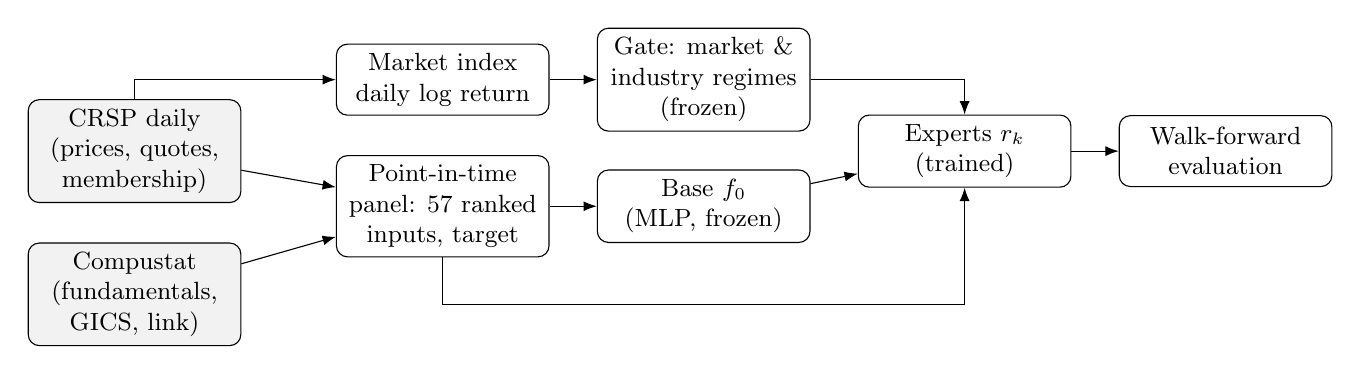
\begin{tikzpicture}[node distance=5mm and 6mm, box/.style={draw,rounded corners,align=center,
  minimum width=27mm,minimum height=9mm,font=\small}, >=Latex]
\node[box,fill=gray!10] (crsp) {CRSP daily\\(prices, quotes,\\membership)};
\node[box,fill=gray!10,below=of crsp] (comp) {Compustat\\(fundamentals,\\GICS, link)};
\node[box,right=12mm of crsp,yshift=-7mm] (panel) {Point-in-time\\panel: 57 ranked\\inputs, target};
\node[box,above=of panel] (mkt) {Market index\\daily log return};
\node[box,right=of panel] (base) {Base $f_0$\\(MLP, frozen)};
\node[box,right=of mkt] (gate) {Gate: market \&\\industry regimes\\(frozen)};
\node[box,right=of base,yshift=7mm] (exp) {Experts $r_k$\\(trained)};
\node[box,right=of exp] (eval) {Walk-forward\\evaluation};
\draw[->] (crsp) -- (panel); \draw[->] (comp) -- (panel);
\draw[->] (crsp.north) |- (mkt);
\draw[->] (panel) -- (base); \draw[->] (mkt) -- (gate);
\draw[->] (base) -- (exp); \draw[->] (gate) -| (exp);
\draw[->] (panel.south) -- ++(0,-6mm) -| (exp.south);
\draw[->] (exp) -- (eval);
\end{tikzpicture}}
\end{center}

Order of work set by the advisor (18 September): data, then compute budget, then parameters; start
experimenting with the base and a generic loss before refining the loss. The reason: the architecture
choices can only be settled once the compute budget is calculated rather than guessed, and the budget
depends on the data.

\section{Data}
\label{sec:data}

\subsection{Sources}

\begin{tabularx}{\textwidth}{@{}>{\raggedright\arraybackslash}p{5cm}X@{}}
\toprule
Source & What it provides \\
\midrule
CRSP daily stock file (CIZ format, release \texttt{ciz202512}) & daily returns including delisting
returns, prices, open/high/low/close, closing bid and ask, volume, shares outstanding, market
capitalisation, index membership spells, index returns \\
CRSP/Compustat Merged (release \texttt{cfz202607}) & quarterly income statement, balance sheet and
cash flow; report dates (RDQ) and filing dates; the dated GICS sector history; the link from
Compustat firms (gvkey) to CRSP securities (PERMNO) \\
\bottomrule
\end{tabularx}

\dec{2026-09-18 and 2026-09-26, Q3, brief 06} CRSP and Compustat through the university replace all free data
(yfinance, Stooq, Wikipedia). Wind remains a possible China extension only.

\begin{whybox}
\begin{itemize}
\item \textbf{Free data is survivorship-biased.} Free sources mostly cover firms that exist today; firms that
  were delisted, merged or went bankrupt disappear, and they are exactly the firms with the worst returns.
  A model trained on survivors learns a world that is too optimistic. CRSP keeps every security and its
  delisting return.
\item \textbf{Point-in-time membership.} CRSP records who was in the S\&P 500 on each day; Wikipedia's list is
  today's list.
\item \textbf{Fundamentals with dates.} Compustat records when each quarter's numbers were reported and filed,
  which is what makes look-ahead-free fundamentals possible.
\item \textbf{Comparability.} CRSP and Compustat are the standard data of the literature this thesis builds on
  (Gu, Kelly \& Xiu; Jensen, Kelly \& Pedersen), so results can be set beside theirs.
\end{itemize}
\giveup{nothing material; the cost is licence discipline (no licensed data leave \texttt{Data/}).}
\end{whybox}

\subsection{Sample period}

\dec{2026-10-05, Q16 (a)} \textbf{2000--2024} (previously 2015--2024). Feature history reaches further back (about
1995, for the five-year windows); the \emph{sample} is what is trained and tested on.

\begin{whybox}
\begin{itemize}
\item \textbf{The research question is about regimes, so the binding quantity is the number of stress
  episodes, not the number of days.} 2015--2024 contains essentially one major crisis (COVID). 2000--2024
  contains 2000--02, 2008--09, 2010, 2011, 2015--16, 2018, 2020 and 2022. A study about behaviour at
  regime transitions cannot rest on one transition, and a stress expert cannot specialise if it has seen
  almost no stress.
\item \textbf{2000 is the earliest start with sector data}: Compustat's dated GICS history begins in mid-1999,
  and the industry block and the industry-level gate need it.
\item \textbf{A fairly homogeneous market structure.} Almost all of the sample is after decimalisation (2001),
  so quoted spreads and short-horizon features mean roughly the same thing throughout.
\end{itemize}
\giveup{the pre-2000 episodes (1987, 1998); in exchange, every data source is consistent over the whole
sample.}
\end{whybox}

\subsection{Universe}

\dec{2026-09-26, brief 06} The \textbf{S\&P 500, point in time}, from CRSP membership spells of index 1000500
(index 1000502 has no constituents), bounds inclusive: 502--508 members a day. Dual-class companies are
kept as two securities.

\begin{whybox}
\begin{itemize}
\item \textbf{Short-horizon signals must be tradeable to mean anything.} At a 5-day horizon, effects in
  microcaps are often unimplementable after costs, and their returns are noisy and partly driven by
  bid--ask bounce. Large caps keep the study close to what a fund could actually trade.
\item \textbf{Clean data.} Quotes, open/high/low prices and fundamentals are essentially complete for S\&P 500
  members, so missing-value handling plays a small role.
\item \textbf{Point in time, so no survivorship.} A stock is in the universe exactly on the days it was in the
  index.
\item \textbf{The closest precedent uses large caps too}, which keeps the comparison meaningful.
\end{itemize}
\giveup{breadth. By the fundamental law of active management, performance grows with the square root of the
number of independent bets, so 500 names offer less than 3,000; size and value spreads are also narrower
inside the S\&P 500.}
\end{whybox}

\subsection{Returns and delistings}

\begin{itemize}
\item Daily log return $\log(1+\text{DlyRet})$.
\item \dec{2026-09-26} \textbf{Delisting returns are already in CRSP's daily return} (checked on the data:
  delisting days carry the delisting return), so they are not compounded in again.
\item A forward window that runs past a delisting is completed by a post-delisting fill, default ``cash''
  (zero return). This default is \textbf{not a decision} and is recorded on every run.
\end{itemize}

\begin{whybox}
Leaving out delisting returns biases returns upward, because delistings for poor performance carry large
negative final returns (Shumway 1997). Adding them a second time would bias them downward. Checking the data
showed the CIZ daily return already contains them, so the right rule is to use it as is. Log returns are
used because they add up across days (a 5-day return is the sum of five daily ones) and are closer to
Gaussian, which suits the likelihood.
\end{whybox}

\subsection{Licence and integrity rules}

CRSP and Compustat data, and anything derived per security, stay in \texttt{Data/}, outside version
control; \texttt{results/} holds aggregate outputs only. No out-of-sample performance number on the real
panel (any date from 2010, and the pilot's validation years) is computed by an assistant; pilot and
scored runs are run by Tom, after pre-registration.

\begin{whybox}
The licence forbids redistribution, and a public repository is redistribution. The integrity rule exists
because the comparison is between small effects: one look at test results that feeds back into a choice
contaminates every later number.
\end{whybox}

\section{Target and horizon}
\label{sec:target}

\subsection{Timing}

Everything is computed at the \textbf{close of day $t$} from information public by then. The gate updates
every trading day, every stock in the universe gets a forecast every day, and the target is the return
from the close of $t$ to the close of $t+5$.

\begin{whybox}
Daily closing data is what CRSP provides, and using one timestamp for features, gate and target makes
look-ahead easy to rule out: every input at $t$ is computed from data up to the close of $t$, and the
target starts after it. The convention assumes trading at the close at which the signal is computed,
which is slightly optimistic; signals concentrated overnight should be checked with a one-day execution
lag.
\end{whybox}

\subsection{Horizon: five trading days}

\dec{2026-10-05, Q21, option B} Daily gate, daily cross-section, \textbf{$h=5$}. Consecutive targets overlap by
four days. The options compared were (A) $h=1$, (B) $h=5$, (C) a monthly target with a daily gate,
(D) monthly gate and cross-section.

\begin{whybox}
\begin{enumerate}
\item \textbf{Enough independent observations.} A monthly horizon leaves too few independent periods to train
  regime-specific experts: in 2015--2024 about 118, of which about 59 in high volatility, and a 5\% rank IC
  at $h=21$ was not significant. Weekly gives about five times as many.
\item \textbf{The regime effect is clearest at this horizon.} A descriptive check (2015--2024, signal
  diagnostics, not model results): one-week reversal had a rank IC of 3.26\% in high-volatility periods
  against 1.29\% in low ones. Short-term reversal is pay for providing liquidity, and it rises when markets
  are turbulent (Nagel 2012). So at a weekly horizon the cross-section demonstrably depends on the market
  state, which is precisely what a regime gate is meant to exploit.
\item \textbf{Less noise than one day.} A one-day return is dominated by noise and bid--ask bounce (the
  closing price jumping between bid and ask, which creates fake reversal; Roll 1984). One-day
  machine-learning strategies on the S\&P 500 have largely decayed since 2010 (Krauss, Do \& Huck 2017;
  Fischer \& Krauss 2018). Five days averages much of this out while keeping short-horizon effects.
\item \textbf{It respects the regime timescale.} Daily regimes typically last 20--50 days, so a 5-day window
  rarely contains a switch, and ``one regime per target window'' is a reasonable approximation. A monthly
  window is as long as a stressed regime and would break it.
\item \textbf{The gate is best identified on daily data}: thousands of daily observations instead of a few
  hundred monthly ones, and daily volatility clustering is what separates the regimes.
\item \textbf{It was already built and audited}: overlap-corrected statistics, purge and a horizon-consistent
  portfolio.
\end{enumerate}
\giveup{direct comparability with the monthly benchmark of Gu, Kelly \& Xiu; independence of
consecutive targets (statistics are overlap-corrected, and the training likelihood is used for
estimation, not inference); and lower turnover than a monthly strategy.}
\end{whybox}

\paragraph{Other horizons (discussed 8 October).} A \textbf{one-day} horizon has real advantages (no overlap,
an exact one-step gate weight, the freshest signals, closer to industry practice) but most of its edge
disappears with a realistic one-day execution delay and five times the turnover. A \textbf{three-day}
horizon is a middle ground, but adds noise and turnover, and its windows sometimes contain a weekend
and sometimes not; there is no evidence it beats five. \dec{2026-10-08, Q21 follow-up} $h=5$ stays primary,
with two robustness additions: an \textbf{IC decay curve} (rank IC of the main signals at
$h=1,2,3,5,10$, on 2000--2006 only) and a \textbf{horizon profile} ($h=1,3,5,10$) for the final model.

\begin{whybox}[Why add these rather than switch]
Whether a shorter horizon is better depends on how fast the signals' predictive power fades. That is a
measurable fact, so it should be measured, not argued; and measured on years before the pilot and the test
period, so that the horizon cannot be chosen on test results. The horizon profile for the final model shows
whether conclusions depend on the horizon, without multiplying the main study.
\end{whybox}

\subsection{Target: the market-neutral return}

\dec{2026-10-01, Q25} For stock $i$ in the universe $\mathcal S_t$, with forward log return
$r_{i,t\to t+5}=\sum_{d=1}^{5}\log(1+r_{i,t+d})$,
\begin{equation}
y_{i,t} \;=\; r_{i,t\to t+5} \;-\; \frac{1}{N_t}\sum_{j\in\mathcal S_t} r_{j,t\to t+5},
\end{equation}
the average running, with equal weights, over the stocks of date $t$ with a valid target. It sums to
zero across stocks every day; the risk-free rate cancels. All reporting is on this basis. \dec{2026-10-05}
The alternatives considered were raw or excess returns, cross-sectionally standardised or ranked returns,
volatility-scaled returns, and factor-residual (CAPM or Fama--French) returns.

\begin{whybox}
\begin{enumerate}
\item \textbf{It is the quantity the question is about.} The thesis asks whether the regime changes
  \emph{which stocks beat which}. The day's average return is the same number for every stock, carries no
  cross-sectional information, and predicting it is market timing.
\item \textbf{It keeps the gate's information and the target's apart.} The gate is fitted on the market
  series. A raw target's largest component is that same market move, so a regime that merely predicts the
  market's direction would look as if it ``helped the experts''. With the common move removed, any gain
  from the gate must come from regime-dependent \emph{cross-sectional} structure. This is the same
  attribution logic that led to freezing the gate.
\item \textbf{It makes the model's assumptions defensible.} The likelihood treats stocks as independent given
  the regime and their characteristics. For raw returns that is badly false: on a $-4\%$ day almost every
  stock falls together. Removing the common move removes the dominant source of dependence.
\item \textbf{Training and evaluation measure the same thing.} Rank IC, decile sorts and equal-weighted
  long-short returns all ignore a number added to every stock on a date, so training on the demeaned
  target spends no capacity on variation the metrics ignore.
\item \textbf{It keeps dispersion}, unlike standardising or ranking. Cross-sectional dispersion rises in stress;
  dividing by it would erase information the experts' noise scales should express.
\item \textbf{It suits a Gaussian likelihood}, unlike ranks.
\item \textbf{Equal weights in the mean} make the target match an equal-weighted, dollar-neutral long-short
  book, and keep it from being driven by a handful of mega-caps. A factor-residual target would bake one
  particular risk model into the label.
\end{enumerate}
\giveup{any claim about market timing (deliberately out of scope) and raw-return reporting.}
\end{whybox}

Note the two different ``markets'' in the pipeline: the target is demeaned by the
\emph{equal-weighted} mean of the universe; the gate and the market-model features use the
\emph{value-weighted} index (Section~\ref{sec:gateinput}). The first defines ``relative'' for an
equal-weighted book; the second measures the state of the market, which large caps drive.

\section{Inputs: the characteristics and how they are prepared}
\label{sec:features}

\dec{2026-10-05, Q26} 40 characteristics and 57 model inputs, in four blocks. Implemented as
\texttt{feature\_set="q26"}; the old 14 price features survive only as \texttt{"legacy14"}.

\subsection{The selection rule}

\textbf{Exactly two representatives per theme} of Jensen, Kelly \& Pedersen (2023, ``JKP''), who cluster 153
published characteristics into 13 themes. Representatives were chosen to be robust in large caps, well
documented, computable from CRSP and Compustat, and not near-copies of each other. PCA on training data is
used only as a redundancy diagnostic.

\begin{whybox}
\begin{itemize}
\item \textbf{A rule, fixed before any result, instead of a search.} Picking features by how well they
  predict would be selection on outcomes. A rule stated in advance cannot be tuned to the data.
\item \textbf{Fewer, well-chosen inputs suit a weak signal and 500 stocks.} Hundreds of characteristics raise
  estimation variance and give the experts more room to relearn general signal (the identification risk of
  Q10). Two per theme covers every documented source of return predictability with about 40 inputs.
\item \textbf{Two, not one, per theme}: one representative can be noisy or fail in a subperiod; two let the
  network combine them, while the fixed count keeps themes balanced so no theme dominates by sheer number
  of inputs.
\item \textbf{Why not PCA as the selector}: principal components mix themes into uninterpretable
  combinations, change from fold to fold, and would have to be re-estimated inside each training block. As a
  diagnostic it still shows whether two representatives are redundant.
\end{itemize}
\end{whybox}

\subsection{Block A: JKP themes (26 characteristics)}

{\small
\begin{tabularx}{\textwidth}{@{}l X X l@{}}
\toprule
Theme & Representative 1 & Representative 2 & Data\\
\midrule
Short-term reversal & 5-day return & 20-day return & CRSP\\
Momentum & 12-month return skipping the last month & price / 52-week high & CRSP\\
Low risk & 21-day volatility & beta (Frazzini--Pedersen) & CRSP\\
Size & log market cap & Amihud illiquidity, 126 days & CRSP\\
Seasonality & same-calendar-month return, years 2--5 back & coskewness with the market, 21 days & CRSP\\
Value & book-to-market & earnings-to-price & both\\
Profitability & quarterly ROE & operating cash flow / assets & Compustat\\
Quality & gross profitability / assets & earnings consistency & Compustat\\
Investment & asset growth & sales growth & Compustat\\
Accruals & operating accruals & total accruals & Compustat\\
Debt issuance & 3-year debt growth & net operating assets / assets & Compustat\\
Low leverage & net debt / market cap & cash / assets & both\\
Profit growth & standardised unexpected earnings (SUE) & revenue surprise & Compustat\\
\bottomrule
\end{tabularx}}

\subsection{Block B: short-horizon market themes (12 characteristics)}

{\small
\begin{tabularx}{\textwidth}{@{}l X X@{}}
\toprule
Theme & Representative 1 & Representative 2\\
\midrule
Volatility dynamics & idiosyncratic volatility, 21 days & volatility shock: 5-day / 60-day volatility\\
Tails and asymmetry & realised skewness, 21 days & maximum daily return, 21 days\\
Volume and liquidity & abnormal volume (today vs trailing average) & quoted spread, 21-day average\\
Price path & overnight (close-to-open) return, 20 days & price / 50-day moving average\\
Earnings timing & announcement expected in the next 5 days (0/1) & trading days since last announcement\\
Return dynamics & variance ratio, 5-day vs 1-day, 60 days & return--volume correlation, 60 days\\
\bottomrule
\end{tabularx}}

\begin{whybox}[Why a short-horizon block]
The JKP themes come from the \emph{monthly} anomaly literature, and 8 of 13 are accounting-based.
Fundamentals barely change from week to week, while the signals known to predict weekly returns are
market-based: price trends, liquidity and volatility dominate the feature importance of Gu, Kelly \& Xiu.
Applying the same two-per-theme rule to six short-horizon themes, each with evidence at a daily or weekly
horizon, matches the inputs to the target's horizon without abandoning the rule. Several were also
confirmed in Tom's own Trexquant work (volatility term structure, the overnight/intraday split, days to
earnings, volume relative to its own average). Levels are expressed as surprises against the stock's own
history (volume, volatility) because a raw level mostly acts as a static tilt.
\end{whybox}

\subsection{Block C: industry (17 inputs) and Block D: flags (2)}

\begin{itemize}
\item 11 \textbf{GICS sector dummies} (0/1); \dec{2026-10-05} GICS from Compustat.
\item \textbf{Industry momentum} (the sector's 12-month return skipping the last month; Moskowitz \&
  Grinblatt 1999) and \textbf{within-industry reversal} (the stock's 20-day return minus its sector's).
\item 4 \textbf{within-sector ranks}: book-to-market, earnings-to-price, quarterly ROE, operating cash
  flow / assets.
\item 2 \textbf{missing-data flags}: one for price/volume inputs, one for fundamentals.
\end{itemize}
Total: $26+12+11+2+4+2=57$ inputs.

\begin{whybox}
\begin{itemize}
\item \textbf{Industries differ in what ``cheap'' or ``profitable'' means.} A bank's book-to-market is not
  comparable with a software firm's. A universe-wide rank of such ratios partly just sorts industries;
  ranking within the sector compares a firm with its peers.
\item \textbf{Sector dummies} let the experts learn sector-specific shifts, which matters more now that the gate
  has an industry level.
\item \textbf{Industry momentum} is a documented, separate source of predictability. \textbf{Within-industry
  reversal} separates a stock's own overreaction from news that moved its whole industry, which is the
  part of short-term reversal most associated with liquidity provision.
\item \textbf{GICS, not ICB}: CRSP stops filling ICB for S\&P 500 members in October 2023, and Compustat's
  GICS history is dated, so each stock gets the sector it had \emph{at the time}, not today's.
\end{itemize}
\end{whybox}

\subsection{Scaling: ranks mapped to $[-1,1]$}

\dec{2026-10-05, Q26 part 2} On each date each characteristic is ranked across the universe (ties get the
average rank) and mapped linearly:
\begin{equation}
x_{i,t} = \frac{2\,(\mathrm{rank}_{i,t}-1)}{N_t-1}-1 \in [-1,1].
\end{equation}
Dummies and flags are not ranked.

\begin{whybox}
\begin{itemize}
\item \textbf{Robust to outliers and scale.} Characteristics like illiquidity or accruals have extreme tails
  that destabilise neural network training; ranks remove them.
\item \textbf{Comparable over time.} A book-to-market of 0.5 means different things in 2000 and 2021; being in
  the top decile means the same thing.
\item \textbf{Only cross-sectional information survives}, which is exactly what the market-neutral target
  measures. This is the convention of Gu, Kelly \& Xiu.
\item \textbf{$[-1,1]$ rather than $[-0.5,0.5]$}: input variance $1/3$ instead of $1/12$, closer to the unit
  variance that standard weight initialisations assume, so the first layer starts in a sensible range.
\end{itemize}
\giveup{the information in absolute levels and in how far apart stocks are, which ranking discards.}
\end{whybox}

\subsection{Missing values: causal handling}

\dec{2026-10-05, Q26 part 3}
\begin{enumerate}
\item Price/volume windows need at least 80\% of their days present.
\item Fundamentals carry the firm's last point-in-time value forward for at most 12 months.
\item Anything still missing is set to 0 after ranking (the median) and the family's flag is set to 1.
\item Rows are no longer dropped for a missing characteristic.
\end{enumerate}

\begin{whybox}
\begin{itemize}
\item \textbf{Never use the future.} Interpolation fills a gap with a later value, which is look-ahead.
  Every rule here uses only data available at $t$.
\item \textbf{Keep every stock.} At forecast time every stock in the universe needs a forecast. A training rule
  that drops incomplete rows trains on a different population from the one it is used on, and missingness
  is not random (new listings, distressed firms).
\item \textbf{Carrying fundamentals forward is barely an imputation}: between two reports the latest filing is
  exactly what the market knows. The 12-month cap stops a stale value standing in for a firm that stopped
  reporting.
\item \textbf{80\% windows}: an average over 16 of 20 days estimates the same quantity with little extra noise;
  requiring all 20 would discard many stock-days around trading halts.
\item \textbf{Zero plus a flag}: in rank space zero is the median, the neutral ``no information'' value, and
  the flag lets the model learn a separate shift for stocks with missing data instead of the fill
  distorting the feature.
\end{itemize}
Four Compustat items (IVAOQ, IVSTQ, MIBQ, PSTKQ) count as 0 when blank in total accruals and net operating
assets: blank there usually means ``none'', and the strict rule left those features on only about 5\% of
rows (79\% after the change).
\end{whybox}

\subsection{Point-in-time fundamentals}

\dec{2026-10-05, Q26 part 5} A quarter's numbers become usable \textbf{one trading day after the later of its
report date and its filing date}; surprises (SUE, revenue surprise) are dated by the report date; flows are
trailing four-quarter sums; market values come from CRSP on day $t$.

\begin{whybox}
\begin{itemize}
\item \textbf{The quarter end is not when investors learn the numbers.} Firms report weeks later, and some items
  appear only in the filing. Using the quarter end plus a fixed lag either leaks information (lag too short)
  or wastes it (too long). Report and filing dates say exactly when the numbers became public.
\item \textbf{One trading day after}, because many announcements come after the close; this removes any
  ambiguity about whether the close of the announcement day could have reacted.
\item \textbf{Surprises by the report date}, because the announcement is the event the market reacts to.
\item \textbf{Trailing four-quarter sums} remove seasonality from flows such as earnings and cash flow.
\end{itemize}
\giveup{restatements: standard Compustat values may be revised after first release (a known limitation).}
\end{whybox}

Every characteristic has a no-look-ahead test: its value at $t$ computed from data truncated at $t$ equals
its value from the full data.

\subsection{What is deliberately not an input}

\begin{itemize}
\item \textbf{Market-wide series} (VIX, rates, FOMC dates, macro data, the market return): identical across
  stocks on a date, so ranking removes them. They belong in the gate. This is also what the closest
  precedent found on its volatility target: appending regime variables to the input made 30 of 30 seeds
  collapse, while feeding them through the gate made none collapse.
\item \textbf{Intraday data, trade counts} (28\% coverage), analyst estimates, options, news: not in the data.
\item Near-copies of included features (position in the 20-day range, high/low ratio, up/down volatility
  ratio).
\end{itemize}

\begin{keybox}{Scoping future alphas}
A new input must be one number per stock per day, known by the close of $t$, varying across stocks; only
its ordering matters. Signals that pay off over 1--10 days fit best. A machine-learning alpha must be
trained inside the same walk-forward folds on out-of-sample predictions only (Improvements item E2).
Inputs added after seeing test results are a forking-paths problem.
\end{keybox}

\section{The model: base, experts and likelihood}
\label{sec:model}

\subsection{Why multilayer perceptrons on a characteristic snapshot}

Each input is a point-in-time vector of characteristics for one stock-day, with no time axis. Base and
experts are MLPs on that vector.

\begin{whybox}
\begin{itemize}
\item \textbf{The input format decides the architecture.} Finance mixture-of-experts papers split into those
  using characteristic snapshots (small MLPs: Gu, Kelly \& Xiu, Ye \& Borde) and those using raw price
  sequences (recurrent or transformer experts). The characteristics already summarise each stock's history
  (momentum, volatility, reversal), so a snapshot model is the natural choice.
\item \textbf{Sequence experts would compete with the gate.} An expert with its own memory of recent market
  history could learn the market state itself and absorb exactly the differences between gates the thesis
  tries to measure.
\item \textbf{Benchmark class and feasibility.} Gu, Kelly \& Xiu establish feed-forward networks as the
  benchmark for this problem, and find shallow networks suffice because the signal is weak. Small MLPs make
  thousands of runs feasible on a laptop.
\end{itemize}
\giveup{the possibility that a sequence model finds patterns the characteristics miss.}
\end{whybox}

\subsection{The base network}

\dec{2026-09-21, Q7} The base $f_0$ is an MLP trained on the training block, then frozen (motivation in
Section~1.3). Its own out-of-sample performance is reported beside every result, the headline quantity is
the \emph{improvement over the base}, and its training protocol is fixed in advance.

\begin{whybox}[Why the base protocol is fixed in advance]
An undertrained base leaves general signal for the experts to pick up and makes them look good; an
overtrained one leaves nothing and makes them look useless. Because the base is shared across gates this
does not bias the comparison \emph{between} gates, but it does set the ``does the residual help'' number,
so it must not be tuned after seeing expert results. A null result is possible (the base may capture
most of a weak signal), and how it is reported is decided before results are seen.
\end{whybox}

\subsection{The experts}

Each expert $r_k$ is an MLP on the same 57 inputs, with a \textbf{zero-initialised output layer}, a learned
\textbf{noise scale} $s_k$, and \textbf{pyramid widths} (first hidden width $w$, each further layer half the
previous).

\begin{whybox}
\begin{itemize}
\item \textbf{Same inputs as the base}: an expert must be able to express a regime-specific version of the
  same characteristic-return relation (for example ``reversal is stronger in stress''), so it needs the
  same characteristics.
\item \textbf{Zero initialisation}: the model starts exactly at the base and moves away only where the data
  justify it. It is tested in the closest precedent: random initialisation lost accuracy and made 13 of
  30 seeds collapse.
\item \textbf{A noise scale per expert}: return dispersion is higher in stress, so each regime's expert should be
  allowed its own uncertainty. This is also what the NLL's variance gain measures.
\item \textbf{Pyramid widths}: the convention of Gu, Kelly \& Xiu (e.g.\ 32--16--8). It reduces the width
  choice to one number, which is what makes ``no width sweep'' workable.
\end{itemize}
\end{whybox}

Open details: \open{Q14} whether a shrinkage penalty on the aggregate correction is used (weight
$\alpha$; zero initialisation is tested in the literature, the penalty is not); \open{audit X-1} the
hidden-layer initialisation; \open{Q8} the first width inside the envelope. The load-balancing penalty used
with trained gates is \textbf{inert} under a frozen gate (its gradient is exactly zero), so it is removed or
documented as such.

\subsection{Depth, width and number of experts}

\dec{2026-09-19, Q11} the full gate-by-expert-depth grid; \dec{2026-10-05} the envelope: depths
\textbf{1--3}, first width \textbf{at most 128}, $K$ \textbf{at most 4}; base depth swept standalone.

\begin{whybox}
\begin{itemize}
\item \textbf{Depths 1--3}: Gu, Kelly \& Xiu find performance peaks at three or four layers and their own
  tests cannot separate any pair of depths; deeper adds cost without evidence of benefit. Depths 4--5
  with width 256 would take about a month of laptop time, the only corner compute rules out.
\item \textbf{Base depth standalone}: the base is trained before any gate exists, so its best depth cannot
  depend on a gate, and sweeping it is a clean replication of Gu, Kelly \& Xiu on this panel.
\item \textbf{$K\le4$}: the data cap the number of regimes (next item), and the closest precedent found
  $K=2$ about as good as $K=4$ and $K=6$ worse and less stable.
\end{itemize}
\end{whybox}

\open{Q18} \textbf{$K$}, the number of regimes, is an input to every gate, not an output, and the usable
count is regime \emph{episodes}, not days; over-specifying a mixture slows estimation dramatically
(Heinrich \& Kahn 2018). With the industry-level gate it may become two numbers (Q28). \open{Q17} what
learning theory can say about network size.

\subsection{The likelihood the experts are trained on}

Each expert defines a Gaussian component centred on the base plus its correction:
\begin{equation}
p(y_{i,t}\mid x_{i,t}) \;=\; \sum_{k=1}^{K}\pi_k(i,t)\,\N\!\big(y_{i,t};\,f_0(x_{i,t})+r_k(x_{i,t}),\,s_k^2\big).
\end{equation}
\dec{2026-10-05, Q24} The objective is the \textbf{per-row} likelihood, one log-sum-exp per stock-day,
\begin{equation}
\ell(\psi) \;=\; \sum_{t}\sum_{i\in\mathcal S_t} w_{i,t}\,\log\sum_{k}\pi_k(i,t)\,
\N\!\big(y_{i,t};\,f_0+r_k,\,s_k^2\big),
\end{equation}
with sample weights $w_{i,t}$ (Section~\ref{sec:weights}), read as the \textbf{composite (independence)
likelihood} of the per-date model in which all stocks on a date share one regime.

\begin{whybox}
\begin{itemize}
\item \textbf{The alternative is the per-date likelihood}, where the product over all of about 500 stocks sits inside the
  sum over regimes. It is the ``literal'' model, but it treats 500 correlated returns as independent
  evidence about the regime, so the realised cross-section can overrule the gate almost completely; in
  simulation it becomes distorted whenever regimes are close.
\item \textbf{The per-row form is consistent}: each term is the exact one-stock marginal of the per-date model,
  so its score has mean zero and the estimates converge to the right values even though cross-stock
  dependence is ignored (composite likelihood theory; Varin, Reid \& Firth 2011).
\item \textbf{It is robust} when the independence assumption fails, which for stock returns it partly does.
\item \textbf{It keeps the gate in charge}, which is the point of freezing it.
\item \textbf{Inference does not rely on it}: significance comes from walk-forward rank ICs with
  overlap-corrected standard errors, so its understated standard errors do no harm.
\end{itemize}
With the industry-level gate the latent is per industry and date, and the per-row form is closer to exact.
\giveup{statistical efficiency (the full joint likelihood would use the dependence between stocks if it
were correctly specified).}
\end{whybox}

\open{Q20} Whether the mixture likelihood stays the training objective at all, against squared or Huber
error on the point forecast or a rank/IC objective. Under the likelihood each expert's gradient is
weighted by its posterior responsibility, which depends on the realised target, so the outcome partly
re-assigns experts after the frozen gate has assigned them; under squared error the gate's weight alone
decides.

\subsection{The point forecast and the NLL}

The forecast used for ranking and portfolios is the mixture mean, equation~\eqref{eq:model}. The NLL is
reported three ways (\texttt{NLL\_single}, \texttt{NLL\_base}, \texttt{NLL\_full}), with the
volatility-only gain next to the correction gain, so that a gain from the experts' different noise
scales is never mistaken for better return forecasts.

\subsection{Planned construction arms}

A construction pilot (one gate held fixed) with five arms: (A) standard MoE, joint training; (B) residual
MoE with the base pre-trained and then unfrozen; (C) residual MoE, frozen base (the design); (D) C with
randomly initialised experts; (E) C with $\alpha=0$. \open{Q6 design half, Q14}

\begin{whybox}[Why run them]
They test the construction instead of assuming it. A versus C checks that the residual advantage found
for volatility survives on returns; B versus C isolates the effect of freezing the base, the one cell
the literature has not tested; D and E separate zero initialisation from the shrinkage penalty.
\end{whybox}

\section{The regime gate}
\label{sec:gate}

\subsection{What the gate does}

The gate answers ``what state is the market (and the stock's industry) in?''. The experts answer
``which stocks beat which in that state?''. The gate is a regime model fitted separately on a few
market-level series and then frozen (\dec{2026-09-21, Q19}; motivation in Section~1.3).

\subsection{The base case: Hamilton's Markov switching model}

A hidden state $z_t\in\{1,\dots,K\}$ follows a Markov chain with transition matrix $A$,
$A_{jk}=\mathbb P(z_t=k\mid z_{t-1}=j)$. Given the state, the market's daily return is Gaussian with a
regime-specific mean and variance:
\begin{equation}
r_t\mid z_t=k\;\sim\;\N(\mu_k,\sigma_k^2).
\end{equation}

\paragraph{How it infers the regime.} Every day the filter combines yesterday's belief, carried forward by
$A$, with how likely today's return is under each regime (Bayes' rule):
\begin{equation}
\xi_{t\mid t}(k)\;=\;\mathbb P(z_t=k\mid\F_t)\;=\;
\frac{f_k(r_t)\,[\xi_{t-1\mid t-1}\T A]_k}{\sum_j f_j(r_t)\,[\xi_{t-1\mid t-1}\T A]_j},
\end{equation}
where $f_k$ is regime $k$'s normal density. Daily means are tiny next to daily volatility, so the regimes
are in practice \textbf{volatility states}: a $-3\%$ day is about 4 standard deviations in a calm regime with
0.7\% daily volatility but 1.5 in a stressed one with 2\%, roughly a thousand times more likely under
stress. The persistence in $A$ stops the gate flipping on single noisy days.

\paragraph{Estimation.} Maximum likelihood by EM (Baum--Welch), from many starting points (24 in the timing
run); regimes relabelled into a canonical order by variance before anything is stored; only \emph{filtered}
probabilities are used, never smoothed ones.

\begin{whybox}
\begin{itemize}
\item \textbf{Hamilton as the base case}: it is finance's native regime model (bull/bear, calm/stress), its
  filter is exact and cheap, and its parameters are interpretable (regime volatilities, expected
  durations). Every other gate is compared against it. Its known weakness, that a Markov chain implies
  memoryless (geometric) regime durations, is part of what the other gates test.
\item \textbf{Mean and variance both switch}, because empirical regimes are separated far more by volatility than
  by mean return.
\item \textbf{Filtered, never smoothed}: the smoothed probability of a date uses data after it. Using it would be
  look-ahead.
\item \textbf{Canonical ordering}: a fitted HMM's labels are arbitrary (``regime 1'' in one fold could be
  ``regime 2'' in the next). Ordering by variance makes ``calm'' and ``stress'' mean the same thing in every
  fold, so experts and decay weights line up.
\item \textbf{Many starting points}: EM finds local optima; several starts, keeping the best, make the fit
  reliable and the optimisation reportable.
\end{itemize}
\end{whybox}

\subsection{The gate types compared}

\begin{tabularx}{\textwidth}{@{}l X l@{}}
\toprule
Gate & What it looks at & Status\\
\midrule
Hamilton (Markov switching) & the market return only & implemented\\
Autoregressive Hamilton & as above, with autoregressive dynamics & implemented\\
Statistical jump model & a feature vector of the market series (volatility over several windows,
downside deviation, trend), clustered with a penalty on switching & to come\\
Wasserstein clustering & the distribution of market returns over a window & to come\\
TVTP Markov switching & regimes from the market return, switching probabilities driven by covariates
(e.g.\ VIX, spreads) & to come\\
\bottomrule
\end{tabularx}

The compute plan counts five gates plus a \textbf{no-regime control} (uniform weights). Jointly trained priors
(soft, hard, top-$k$, Gumbel) and a backpropagation-trained HMM are kept as \textbf{baseline arms}. \open{Q13}
whether a recurrent (GRU) gate is added.

\begin{whybox}[Why these gates]
Each gate embodies a different idea of what a regime is, which is what makes the comparison informative:
\begin{itemize}
\item \textbf{Hamilton}: a latent Markov process of market volatility; the classic econometric view.
\item \textbf{Jump model}: regimes as persistent clusters, with the switching penalty acting like a turnover
  cost (a gate that flips daily implies a strategy that trades daily).
\item \textbf{Wasserstein}: regimes as shapes of the return distribution, with no economic theory behind it;
  it serves as the ``no economics'' control: if a purely geometric gate does as well, the economic content
  of the others adds nothing.
\item \textbf{TVTP}: switching driven by observable conditions (volatility, spreads, sentiment); the gate
  whose equation is itself an economic hypothesis.
\item \textbf{No-regime control}: the same model with uniform weights; the difference between it and any gate is
  the honest measure of what gating contributes.
\end{itemize}
\end{whybox}

\subsection{What the gate is fitted on}
\label{sec:gateinput}

\dec{2026-10-08, Q23} The \textbf{CRSP value-weighted index of the S\&P 500 universe} (1000500), daily total
return, as a \textbf{log return}. French's Mkt-RF stays registered as a robustness check.
\impl{brief 10 B}

\begin{whybox}
\begin{itemize}
\item \textbf{One market definition.} The universe is the S\&P 500 and the market-model features (beta,
  idiosyncratic volatility, coskewness) use this index. The regime should describe the market the experts
  trade in, not the whole US market including small caps.
\item \textbf{Same source, no lag}: from the same licensed CRSP release; no external file published with a
  delay.
\item \textbf{Precedent}: Nystrup, Madsen \& Lindstr\"om (2017), whose method the gate's memory follows, fit
  their HMMs on S\&P 500 daily log returns.
\item \textbf{The risk-free rate is immaterial} (about 0.005\% a day against 1\% volatility), so a raw return
  does as well as an excess return.
\item \textbf{Log returns} add up over days and are closer to the Gaussian the model assumes.
\end{itemize}
\giveup{the literature's most common series (French's Mkt-RF), kept as a robustness check.}
\end{whybox}

What the gate does \emph{not} see, and why:
\begin{itemize}
\item \textbf{Stock characteristics}: after ranking they look the same every day, so they say \emph{which
  stocks}, not \emph{what state the market is in}. They belong in the experts. Keeping them out of the gate
  also keeps the regime a property of the market, not of individual stocks.
\item \textbf{A market-neutral series}: the market minus the market is zero. The market's own moves and
  volatility are the regime signal; neutralising applies to the target only.
\end{itemize}

\open{Q29} A gate variant on the vector of daily \textbf{factor returns} (market, size, value, momentum), so
regimes describe how the cross-section behaves; motivated by momentum crashes in falling-volatility
rebounds (Daniel \& Moskowitz 2016).

\subsection{The gate weight for a five-day target}

\dec{2026-10-05, Q27} The \textbf{average over the target window of the 1- to 5-step-ahead regime
probabilities}:
\begin{equation}
\pi(t) \;=\; \frac{1}{h}\sum_{j=1}^{h}\xi_{t\mid t}\T A^{j}, \qquad h=5 .
\end{equation}

\begin{whybox}
\begin{itemize}
\item \textbf{The target spans five days, and the regime can move during them.} The weight that matches a
  5-day return is the expected share of those five days spent in each regime, and that is exactly this
  average. It makes the model's expected 5-day return exact.
\item \textbf{The alternatives answer the wrong question.} The filtered probability describes today, which is
  not in the target window; the one-step prediction describes only the first day of the window.
\item \textbf{It nests the simple case}: at $h=1$ it equals the one-step prediction.
\item \textbf{Same weight in training and forecasting}, so experts are trained on the weights they will be used
  with.
\end{itemize}
In practice it differs from the filtered weight by 0.055 on average (maximum 0.10) on 2015--2024.
\end{whybox}

\subsection{The filter runs through the purge gap}

\dec{2026-10-08, Q22} The gate's parameters are fitted on the training block only, but its filter runs over
every trading day, including the 5 purged days before each test year. \impl{brief 10 A}

\begin{whybox}
\begin{itemize}
\item \textbf{The purge exists for labels, not information.} The gap days are dropped from training because
  their 5-day targets reach into the test year. Their market returns, however, are public by the first test
  date, and a live trader's filter would have processed them. Skipping them makes the backtest less
  realistic, not safer.
\item \textbf{It removes a mis-specification}: $A$ describes one trading day; skipping the gap made one step of
  $A$ bridge six days at every fold boundary.
\item \textbf{The window-average weight and the regime-clock decay start from the filtered probability}, so the
  state at the start of each test year should be exact.
\end{itemize}
The effect is small (largest change 0.008 in a regime probability on the smoke panel); this is a correctness
point.
\end{whybox}

\subsection{The gate's memory}

\dec{2026-10-05, Q16 (d)(e)} \textbf{Regime-clock forgetting}: a weighted Baum--Welch in two passes (an
unweighted fit, then weights from each regime's own clock, then weighted M steps; each regime's emission
parameters use its own clock, transitions out of regime $j$ use $j$'s). The half-life is chosen in the pilot
by the one-step predictive log-likelihood of the market series.

\begin{whybox}
\begin{itemize}
\item \textbf{Why not the full history with equal weights}: the gate's parameters drift. Nystrup, Madsen \&
  Lindstr\"om (2017) find a two-state HMM's parameters on daily S\&P 500 returns change well beyond
  estimation noise, and adaptive estimation forecasts better. A bias--variance trade-off applies to the
  gate just as to the networks.
\item \textbf{Why not plain calendar forgetting}: a short calendar memory can forget the stress state entirely
  during a long calm spell (2012--2019), exactly when it is needed next. Regime-clock forgetting ages each
  regime's data only by new experience of that regime, so the last crisis keeps its weight until the
  next one.
\item \textbf{Why choose the memory by predictive likelihood}: that is the gate's own job (describing the
  market series). Choosing it by the experts' loss would let the experts shape the gate, a partial return to
  joint training. It also gives every gate type the same tuning budget.
\end{itemize}
\end{whybox}

\subsection{The industry-level gate}
\label{sec:industrygate}

\begin{decbox}{Decided 2026-10-08 (Q1): the gate is partly stock-specific, at the industry level}
Each stock's gate weight combines the \textbf{market regime} (shared by all stocks) with a regime of its
\textbf{industry}. Stocks in the same sector on the same date share a weight; stocks in different sectors
can differ. Both parts are fitted separately and frozen.
\end{decbox}

\begin{whybox}
\begin{itemize}
\item \textbf{Industries have their own regimes.} Energy in 2014--16, banks in 2008 and 2023, technology in
  2000--02 and 2022 were in stress while much of the market was calmer. A market-wide gate gives every
  stock the same state and cannot express this.
\item \textbf{Why the industry level and not each stock}: a single stock's ``regime'' is mostly its own news
  (earnings, deals), which the experts already see through volatility and event features; a per-stock gate
  would duplicate the inputs and turn the gate into a per-stock router, which moves the thesis away from
  regime processes. An industry aggregates enough stocks to have a genuine state with an economic cause
  (oil prices, interest rates for banks), and there are few enough sectors (11) to estimate each reliably.
\item \textbf{The market regime stays at the core}, which is the part best supported by the literature and by
  the descriptive checks, and keeps the gate comparison intact.
\item \textbf{Cost is small}: frozen weights are looked up per row, so network training is unchanged; only the
  gate fits multiply (about 29\,s each).
\end{itemize}
\giveup{the simplicity of one weight vector per date, and a larger design space that has to be settled
(Q28). The advisor should hear this explicitly, since it widens the object of study.}
\end{whybox}

\begin{openbox}{Open (Q28): how the industry-level gate is implemented}
Candidate forms:
\begin{enumerate}[label=(\alph*)]
\item \textbf{Factorial gate}: two independent hidden chains (market and sector), one expert per pair of
  states (Ghahramani \& Jordan 1997):
  \[\pi_{(k,l)}(i,t)=\pi^{\text{mkt}}_k(t)\,\pi^{\,s(i)}_l(t),\]
  with $s(i)$ the stock's sector; $2\times2$ states gives 4 experts, inside the envelope.
\item \textbf{Coupled chains}: the sector chain's transitions depend on the market state.
\item \textbf{Sector gate only}, with the market regime entering another way.
\item \textbf{Pooled industry chains}: shared regime definitions and transition matrix, each sector with its
  own chain; one fit per fold.
\end{enumerate}
Sub-questions: sector-relative or raw sector returns; 11 sectors or finer groups; states per level (Q18);
industry versions of each gate type; identification against the industry inputs (Q10); a descriptive
check of how often a sector is stressed while the market is calm.
\end{openbox}

\section{Training scheme}
\label{sec:training}

\subsection{Order of fitting within a fold}

For each fold (training block, test year):
\begin{enumerate}
\item Fit the gate on the training block; freeze it; run its filter forward over the gap and the test year.
\item Fit the base with calendar-decay weights; freeze it; cache its predictions.
\item Train the experts with regime-clock weights and the frozen gate weights.
\item Predict the test year.
\end{enumerate}

\begin{whybox}[Why this order]
Each step only uses what the previous ones froze. The gate comes first because the experts' sample weights
are computed from its filtered probabilities (the regime clock) and its weights enter their likelihood.
The base comes before the experts because they learn corrections to it. Nothing fitted later can change
anything fitted earlier, which is the frozen design in procedural form.
\end{whybox}

\subsection{Windows and folds}

\dec{2026-10-05, Q16 (b)} \textbf{Expanding window, never rolling.}

\begin{whybox}
\begin{itemize}
\item \textbf{A rolling window can contain no crisis at all.} A two-year window in 2014 has no stress episode,
  so the stress expert has nothing to learn from, and by 2020 the model cannot recognise that conditions
  resemble 2008 because 2008 has left the window.
\item \textbf{Adaptation is the gate's job, not the window's.} In a regime-gated model the gate handles
  changing conditions; the base should have the longest possible sample for a low-variance estimate of the
  average relation.
\item \textbf{Old data is down-weighted, not dropped} (Section~\ref{sec:weights}), which keeps the benefits of
  recency without losing the rare episodes.
\end{itemize}
\giveup{the protocol of the closest precedent (a rolling 504-day window).}
\end{whybox}

\dec{2026-10-05} \textbf{Test period 2010--2024, refitted annually: 15 folds}, each re-fitting gate, base
and experts on the expanding block from 2000 to the year before.

\begin{whybox}
\begin{itemize}
\item \textbf{Why 2010 and not 2008}: every setting must be chosen on data before the first test year. A 2008
  start leaves only the calm years 2005--07 for tuning a regime model. A 2010 start lets the pilot see the
  2008 crisis, every training block contains two crises, and the test period still has six stress
  episodes, including COVID, the sharpest transition test. 2008 itself can still be tested out of sample
  by leave-one-episode-out.
\item \textbf{Why annual}: the filter already updates the regime every day, so the model reacts daily;
  refits only update slow parameters. Quarterly refits would cost four times as much for little gain, and
  Gu, Kelly \& Xiu also refit annually with an expanding window.
\end{itemize}
\end{whybox}

A \textbf{5-day purge} separates training and test blocks (the gap's labels are dropped; the gate's filter
still sees its returns). \open{Q16 (c)} \textbf{Leave-one-episode-out}, as headline or robustness.

\begin{whybox}[Why the purge]
A training row from four days before the test year has a target that ends inside the test year. Keeping it
would let test-period returns leak into training. Removing $h$ days removes every such overlap.
\end{whybox}

\subsection{Sample weights: one memory per component}
\label{sec:weights}

\dec{2026-10-05, Q16 (d)(e)}

{\small
\begin{tabularx}{\textwidth}{@{}l X X X@{}}
\toprule
Component & Estimates & Main risk & Memory\\
\midrule
Base & the average cross-sectional mapping & bias: structural drift shows here & calendar exponential
decay, long half-life\\
Experts & regime-specific mappings & variance for rare regimes & regime-clock decay\\
Gate & regime dynamics of the market & both & regime-clock forgetting\\
\bottomrule
\end{tabularx}}

\begin{whybox}[Why weight at all, and why differently per component]
This is a bias--variance trade-off. Old data adds \emph{bias} because markets change: anomalies weaken after
publication (McLean \& Pontiff 2016) and as markets become more liquid (Chordia, Subrahmanyam \& Tong 2014).
Dropping old data adds \emph{variance} in a setting where the signal is tiny, and the optimal weights after a
structural break are smaller but not zero (Pesaran \& Timmermann 2007). Exponential down-weighting sits
between the expanding window (no decay) and a rolling window (a hard cut-off). The three components face
the trade-off differently, so each gets its own memory.
\end{whybox}

\paragraph{Calendar decay (base).} A row $a$ trading days old gets weight $w_a=\rho^{a}$ with $\rho=2^{-1/H}$.
The Kish effective sample size then tends to $(1+\rho)/(1-\rho)$, about 2.9 half-lives, however long the
history.

\begin{whybox}
The base estimates the average relation across all regimes, which is where slow structural drift shows
most, and every day informs it, so ordinary recency weighting fits. The half-life is long because the
signal is weak and the effective sample shrinks fast as the half-life shortens.
\end{whybox}

\paragraph{Regime-clock decay (experts; Tom's construction).} A row's age is the amount of \emph{later
experience of the same regime}, counted with the gate's filtered probabilities:
\begin{equation}
w_s(t)=\sum_{k=1}^{K}\xi_{s\mid s}(k)\,\rho^{\,n_k(s,t)},\qquad
n_k(s,t)=\sum_{u=s+1}^{t}\xi_{u\mid u}(k),\qquad \rho=2^{-1/H}.
\end{equation}
A regime occupying a share $p$ of days has a calendar half-life of about $H/p$: with $H=500$ regime-days,
about 2.8 years for a calm regime (70\% of days), 6.6 years for stress (30\%), decades for a rare crisis
state. \open{minor} mixture form (default) or a per-expert clock.

\begin{whybox}
\begin{itemize}
\item \textbf{Calendar decay would erase the crises}: with a two-year half-life, 2008 data carries about 1.6\%
  weight by 2020. The crisis regime has the least data and almost all of it is old, so calendar decay
  starves exactly the expert that needs history most.
\item \textbf{Regime-clock decay resolves the conflict between ``markets drift'' and ``regimes recur''}: in a
  long calm spell, calm data turns over quickly (drift is tracked) while the last crisis keeps its weight
  because no newer crisis experience has replaced it. After a cluster of crises, older crisis data fades.
\item \textbf{Nothing is hand-labelled}: the gate's own filtered probabilities do the work, with no look-ahead
  and no choice of ``important periods'' that could be snooped.
\end{itemize}
The closest precedent for weighting history by regime rather than calendar time is Mulliner, Harvey, Xia,
Fang \& Van Hemert (2025). Measuring age in regime time with filtered probabilities is this study's own
construction.
\end{whybox}

In the likelihood each row's term is multiplied by its weight (a weighted composite likelihood): scores
stay unbiased, so the weights change efficiency, not consistency.

\subsection{The pilot: every setting chosen once}

\dec{2026-10-05} A pilot on three folds with \textbf{validation years 2007, 2008 and 2009}, which never touches
2010 or later, chooses once: the half-lives (from a small grid always including equal weights) and the gate
memory; learning rate, weight decay and batch size; the training length as a fixed number of steps.
Settings other than the gate's memory are chosen by a \textbf{regime-balanced validation loss}, each row
reweighted by
\begin{equation}
v(s)=\sum_{k}\frac{\bar w_k(s)}{M_k},
\end{equation}
where $\bar w_k(s)$ is the window-average gate weight and $M_k$ its mean over the validation block.

\begin{whybox}
\begin{itemize}
\item \textbf{Choose once, before the test period}: tuning in every fold or on test data would let test results
  shape the model (Q15). One lock file, written before any test year is touched, is the pre-registration.
\item \textbf{Why 2007--2009}: the validation years include the calm run-up, the crisis and the recovery, so
  settings are chosen on a full cycle.
\item \textbf{Why regime-balanced}: about 70\% of days are calm, so an unweighted validation loss would choose
  settings that serve calm markets and ignore stress, the very thing the gate exists for. Balancing makes
  every regime count equally.
\item \textbf{Equal weights always in the grid}, so ``decay does not help'' is a possible, reportable outcome, and
  the undecayed protocol of Gu, Kelly \& Xiu is always available as a reference.
\end{itemize}
\end{whybox}

\subsection{Main study: frozen settings, full blocks}

\dec{2026-10-05}
\begin{itemize}
\item \textbf{No held-out validation tail and no per-fold early stopping}; fallback to regime-balanced early
  stopping if the pilot's best step count drifts across its folds.
\item \textbf{Train on every day} under a fixed step budget.
\item \textbf{Fresh initialisation every fold}; no warm starts (fallback: shrink-and-perturb).
\item \textbf{Paired seeds}: 10 per grid cell, 30 for the primary cell, final count from the pilot.
\item \textbf{One process per performance core}, large batches, features built once, base cached.
\end{itemize}

\begin{whybox}
\begin{itemize}
\item \textbf{No validation tail}: holding out the last 20\% of each block would withhold the most recent, most
  heavily weighted data from training. Decay keeps the effective sample roughly stable as the window grows,
  so a step budget chosen in the pilot should transfer; the pilot checks this.
\item \textbf{Every day}: under a fixed step budget, thinning to every fifth day saves no compute; overlapping
  rows still add information because the price features change daily, and overlap only affects standard
  errors, which are corrected.
\item \textbf{Fresh starts}: warm-started networks generalise worse (Ash \& Adams 2020); a warm start would also
  make corrections relative to last year's base, breaking the zero-initialised residual design, and would
  tie the folds together.
\item \textbf{Paired seeds}: the quantity of interest is the \emph{difference} between gates. Running every arm on
  the same seeds makes much of the training noise common to both arms, so it cancels in the difference
  (common random numbers). The seed count is set by the measured noise, not guessed.
\item \textbf{Process parallelism}: measured on the laptop, one thread per run with ten runs in parallel gives
  about seven times the throughput; extra threads inside one run give nothing.
\end{itemize}
\end{whybox}

\section{Evaluation}
\label{sec:evaluation}

\subsection{Metrics}

\begin{itemize}
\item \textbf{Rank IC} (Spearman correlation across stocks between forecasts and realised market-neutral 5-day
  returns, per test date), reported as its mean and ICIR; t-statistics with \textbf{Hansen--Hodrick} standard
  errors at lag 4. \dec{2026-09-26, audit E-2}
\item \textbf{Negative log-likelihood}, three ways (\texttt{NLL\_single}, \texttt{NLL\_base},
  \texttt{NLL\_full}), with the volatility-only gain next to the correction gain.
\item \textbf{A horizon-consistent long-short book}, equal-weighted and dollar-neutral; non-overlapping or
  staggered. \open{default scheme}
\item \textbf{Stability across seeds}: dispersion of rank IC and the count of seeds below a stated IC threshold.
\item \textbf{Regime-conditional results}: by regime and in transition windows.
\end{itemize}

\begin{whybox}
\begin{itemize}
\item \textbf{Rank IC} measures what the thesis is about, the ordering of stocks, and is robust to outliers
  and to the scale of the forecasts. It is the standard metric for cross-sectional signals and is invariant
  to the market-neutral demeaning.
\item \textbf{Hansen--Hodrick}: daily 5-day targets share four days, so consecutive ICs are correlated and naive
  t-statistics are too large. Hansen--Hodrick corrects exactly for overlap of known length, and in our
  simulation it had better size than Newey--West.
\item \textbf{Three NLLs}: a mixture can lower the NLL just by giving stressed regimes a wider distribution,
  without forecasting returns any better. Separating the variance gain from the correction gain stops that
  being mistaken for predictive skill.
\item \textbf{The long-short book} translates IC into an economic quantity. Equal-weighted and dollar-neutral, it
  matches the target's definition; horizon-consistent, so overlapping signals are not double-counted.
\item \textbf{Stability}: in the closest precedent, the largest differences between designs were in how many
  seeds failed, not in average accuracy. Their failure criterion is volatility-specific, so a returns
  version is defined in advance.
\item \textbf{Regime-conditional results}: the theory predicts gains where the regime matters (stress and
  transitions). The precedent's gain was concentrated in sustained high volatility and was weak at
  transitions; a regime process with persistence and transition dynamics is aimed at exactly that gap.
\end{itemize}
\end{whybox}

\subsection{Reporting additions (decided 2026-10-09)}

\dec{2026-10-09, Q9 update} Four additions to every arm's evaluation (gates, control, base, baselines), adopted after
reviewing the LightGBM pipeline in \texttt{OP model/lgbm}. They are reporting only and were fixed before any
test-period number was computed. \impl{brief 12}
\begin{enumerate}
\item \textbf{Long leg against short leg}: the long-short spread split into the long leg (mean market-neutral return of
  the top quantile) and the short leg (minus the mean of the bottom quantile), plus the rank IC computed separately
  within the upper and lower halves of the forecast distribution.
\item \textbf{Decile monotonicity}: mean return by forecast decile, and the monotonic relation test of Patton \&
  Timmermann (2010), with a stationary bootstrap.
\item \textbf{By calendar year and named episode}: 2010--2024 year by year, and eight episodes fixed in advance:
  euro debt and flash crash 2010; US downgrade 2011; China devaluation and oil 2015--16; the 2018 fourth-quarter
  sell-off; the COVID crash; the 2020 rebound; the 2022 bear market; the 2023 regional-bank stress.
\item \textbf{Execution lag}: a setting \texttt{execution\_lag}; with lag $L$ the forecast made at the close of $t$ is
  scored against the return over $(t+L,\,t+L+h]$. Evaluation only; every headline table at $L=0$ and $L=1$.
\end{enumerate}

\begin{whybox}
\begin{itemize}
\item \textbf{Legs}: in the LightGBM pipeline nearly all the edge sat in the short leg (IC 0.028 against 0.004). If the
  regime gain lives only in the short leg during stress, that changes how it could be used (shorting is costlier and
  constrained).
\item \textbf{Monotonicity}: a good spread can come from one extreme decile. A forecast that orders stocks well should
  raise returns steadily from decile 1 to 10.
\item \textbf{Years and episodes}: one headline number can hide an edge that lived in one year. Fixing the episode
  dates now means they cannot be chosen to flatter a gate.
\item \textbf{Execution lag}: the book assumes trading at the close at which the signal is computed. The IC decay curve
  showed several signals carry most of their information in the first two or three days, so a one-day delay is the
  honest check.
\end{itemize}
\end{whybox}

\paragraph{Turnover without trading.} Nothing is traded, but the evaluation builds a paper long-short book every
rebalance, so its turnover, $\tfrac12\sum_i|w_{i,t}-w_{i,t-1}|$, measures how stable the forecasts' rankings are (0: same
names; 1: whole book replaced). A gate that switches regime moves every stock's expert weights at once, so its
forecasts jump and turnover spikes; this makes turnover an assumption-free measure of how usable each gate's forecasts
are. A cost-adjusted return additionally needs an assumed cost per unit traded, which is why it stays with
\open{Q9 (c)}.

\open{Q9} Which metric family is primary: forecast accuracy or portfolio performance. In Gu, Kelly \& Xiu
the two families favour different depths, so the primary family must be fixed in advance.

\subsection{Diagnostics of what the gate contributes}

\open{Q10} The frozen base buys identifiability of the correction term, not of what it contains. Two
failure modes: the base underfits and the experts relearn general signal; or all experts converge to the
same correction and the gate is decorative. Planned diagnostics:
\begin{enumerate}
\item \textbf{Decomposition} of the correction into a gate-independent part (mean expert output) and a
  gate-conditional part, with each part's share of explained variation.
\item \textbf{Gate permutation test}: replace the fitted gate weights by uniform weights or weights from random
  other dates and build a null distribution.
\item \textbf{Expert-weight diagnostic} and the \textbf{effective sample per expert}.
\item A \textbf{variance decomposition} of gate weights across dates and across industries within a date (now
  meaningful with the industry-level gate).
\end{enumerate}

\begin{whybox}[Why these diagnostics]
A good number for the mixture is not evidence that \emph{regimes} helped: the experts might simply be fixing
what the base missed, identically in every regime. The decomposition and the permutation test answer the
question the thesis actually asks, ``does it matter \emph{which} regime the gate says we are in?''. The
permutation test needs no extra data and is the strongest single piece of evidence available.
\end{whybox}

\subsection{Baselines}

\open{Q12} Candidates: a capacity-matched single network; a network matched to one expert; a penalised
linear model; gradient-boosted trees (e.g.\ LightGBM); the no-gate mixture; jointly trained priors.

\begin{whybox}[Why these candidates]
Every claim is relative to a baseline. The capacity-matched network separates ``the gate matters'' from
``more parameters help''; the linear model shows the nonlinear machinery does anything at all; trees answer
the predictable referee question (trees are strong on tabular data, and Gu, Kelly \& Xiu cannot separate
networks from trees statistically); the no-gate mixture is the cleanest measure of gating itself.
\end{whybox}

\subsection{Multiple testing and pre-registration}

\open{Q15} The test set may be reused across models; what biases results is \emph{using test performance to
choose}. Seeds are not multiple testing; configurations are (about 18 gate-by-depth cells plus construction
arms). Open: the formal correction (e.g.\ Benjamini--Hochberg) and the pre-registration document.

\begin{whybox}[Why this matters so much here]
The differences between gates are likely small. Picking the best of 18 noisy estimates and reporting it as
if chosen in advance can create a ``winner'' out of noise alone. Locking every setting in the pilot,
nominating the primary cell in advance and correcting for the number of comparisons is what makes the
final ranking of gates believable.
\end{whybox}

\section{Pre-pilot descriptive diagnostics (2000--2006)}
\label{sec:diagnostics}

Three descriptive studies were run on the earliest years of the sample before any model was scored. They
test the premises of the design (the horizon, regime dependence of the cross-section, industry regimes)
on data the pilot and the test period never use.

\begin{keybox}{Rules that applied to all three}
\begin{itemize}
\item \textbf{Hard date guard 2000-01-01 to 2006-12-31.} Forward windows end by 2006-12-31, so the last scored
  date moves back by $h$; no 2007 return was read. The pilot's validation years (2007--2009) and the test
  period (2010--2024) are untouched.
\item \textbf{Descriptive only.} No result feeds back into a design choice: not the horizon (unless the evidence
  overturned it), not $K$ (Q18), not the features (Q26), not the industry-gate form (Q28).
\item \textbf{Readings written down before each run}, including what a negative result would mean.
\item Code written and tested on synthetic data by Claude Code (briefs 10 C and 11); real runs by Tom.
\end{itemize}
\end{keybox}

\begin{whybox}[Why run diagnostics before the pilot]
The thesis rests on two premises: that a five-day horizon is the right place to look, and that the cross-section
of returns depends on the market's regime. Both can be checked cheaply on years that play no other role. Running
them first means a failed premise is discovered before compute is spent, and a confirmed one enters the thesis
as evidence fixed in advance rather than as a story told after the results.
\end{whybox}

\subsection{The IC decay curve: is five days the right horizon?}

\paragraph{Method (brief 10 C).} For 16 signals (the two reversal and two momentum characteristics of the JKP
block and the 12 short-horizon characteristics), the daily cross-sectional rank IC against the market-neutral
forward return at $h = 1, 2, 3, 5, 10$, averaged over 2000--2006, with Hansen--Hodrick t-statistics at lag $h-1$.

\paragraph{How to read it.} If a signal predicts every day of the next $h$ equally, its IC grows like $\sqrt h$
(a factor 2.2 at $h=5$, 3.2 at $h=10$) and its overlap-corrected t-statistic stays roughly flat. If it predicts
only the next day, its IC shrinks like $1/\sqrt h$ and its t-statistic falls. So a falling t-statistic means the
signal's information is fading.

\begin{center}
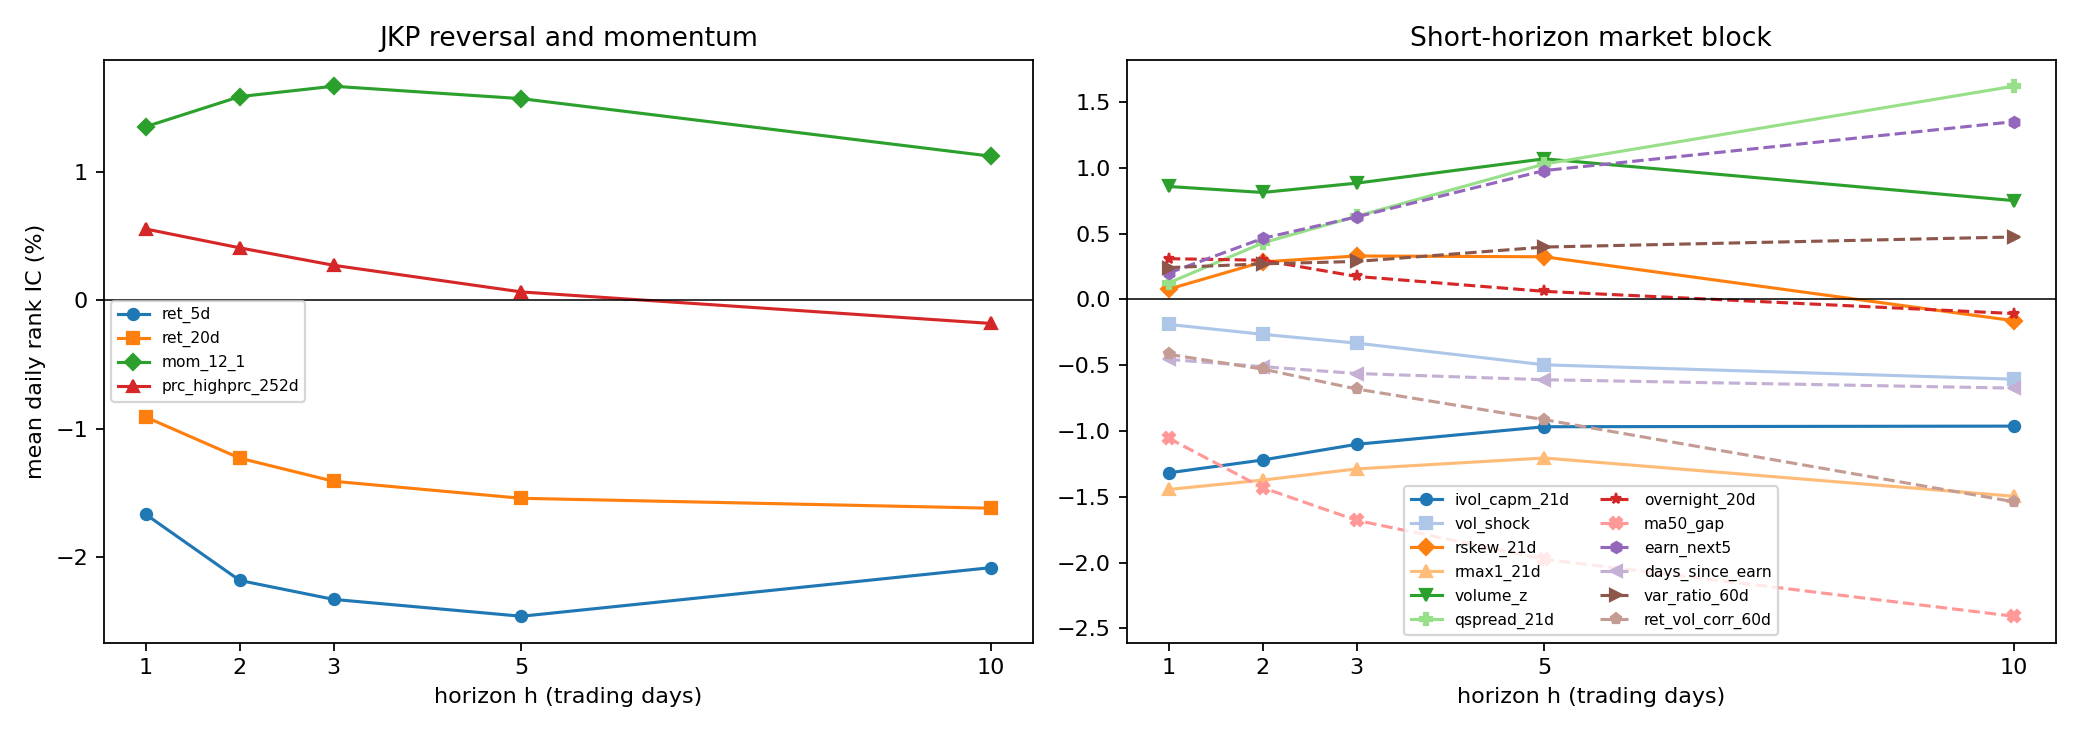
\includegraphics[width=\textwidth]{fig/ic_decay_redrawn.png}
\end{center}

{\small
\begin{tabular}{@{}lrrrrl@{}}
\toprule
Signal & IC $h{=}1$ & IC $h{=}5$ & IC $h{=}10$ & $t$ ($h{=}5$) & Shape\\
\midrule
\texttt{ret\_5d} (one-week reversal) & $-1.67$ & $-2.46$ & $-2.08$ & $-4.21$ & builds to 5, then done\\
\texttt{volume\_z} (abnormal volume) & $+0.86$ & $+1.07$ & $+0.75$ & $4.05$ & peaks at 5, most robust\\
\texttt{mom\_12\_1} (momentum) & $+1.36$ & $+1.57$ & $+1.12$ & $1.43$ & peaks at 3, fades\\
\texttt{ivol\_capm\_21d} & $-1.32$ & $-0.97$ & $-0.96$ & $-0.90$ & strongest next day\\
\texttt{rmax1\_21d} (max return) & $-1.44$ & $-1.20$ & $-1.50$ & $-1.14$ & flat IC, $t$ falls\\
\texttt{ret\_20d} (one-month reversal) & $-0.91$ & $-1.54$ & $-1.62$ & $-1.97$ & still building\\
\texttt{ma50\_gap} & $-1.06$ & $-1.97$ & $-2.41$ & $-2.33$ & slow, close to $\sqrt h$\\
\texttt{ret\_vol\_corr\_60d} & $-0.42$ & $-0.91$ & $-1.54$ & $-1.92$ & slow\\
\texttt{qspread\_21d} (spread) & $+0.13$ & $+1.03$ & $+1.62$ & $1.80$ & nothing next day, accrues\\
\texttt{earn\_next5} & $+0.20$ & $+0.98$ & $+1.35$ & $3.25$ & the event falls in the window\\
\texttt{days\_since\_earn} & $-0.46$ & $-0.61$ & $-0.67$ & $-1.51$ & weak\\
\texttt{prc\_highprc\_252d} & $+0.56$ & $+0.07$ & $-0.18$ & $0.06$ & gone by 5\\
\bottomrule
\end{tabular}}

ICs in percent. Volatility shock, realised skewness, overnight return and variance ratio have $|t| < 1.3$ at every
horizon.

\paragraph{Findings.}
\begin{itemize}
\item \textbf{The strongest signal peaks at $h=5$.} One-week reversal builds to five days and adds nothing after;
  abnormal volume also peaks at five.
\item \textbf{Fast signals} (idiosyncratic volatility, maximum return, momentum, the 52-week high) lose IC and
  t-statistic by five days: most of their information is in the first two or three days.
\item \textbf{Slow signals} (distance from the 50-day average, the spread, the earnings dummy, one-month reversal)
  keep building to ten days; a one-day target would miss them.
\item \textbf{Nothing points to three days beating five.}
\end{itemize}

\paragraph{Caveats.} 80 tests (16 signals $\times$ 5 horizons): under Bonferroni ($|t|>3.4$) only one-week reversal
and abnormal volume ($h\le5$) and the earnings dummy ($h=10$) clear the bar. Regimes are pooled: 2000--2006 mixes the
2000--02 bear market with the calm of 2003--06, so a signal with opposite signs in calm and stress averages to near
zero (the motivation for the next study).

\begin{decbox}{Decided 2026-10-09 (Q21 follow-up)}
$h = 5$ confirmed; the horizon question is closed. The Q26 inputs are unchanged.
\end{decbox}

\begin{whybox}[Why the weak signals were not dropped]
The feature list was fixed by a rule (two representatives per theme) precisely so that it would not be chosen on
outcomes. Pruning signals for weak pooled ICs would turn a rule-based selection into an outcome-based one, even on
pre-pilot years. And a pooled IC near zero is exactly what a signal whose sign depends on the regime would show,
which is a reason for a regime gate, not against the signal.
\end{whybox}

\subsection{Market regimes on 2000--2006}

\paragraph{Method (brief 11 A).} The Hamilton gate fitted on the CRSP S\&P 500 index's daily log return over
2000--2006 with equal weights (the pilot had not yet chosen the memory), $K=2$ as the main case and $K=3$ as a check;
only filtered probabilities; for each horizon the window-average gate weight of Q27. The parameters are estimated on
the whole span, so the probabilities are causal in the data but not in the parameters: an in-sample description,
not a forecast. A parameter-free check: ``stress'' when the trailing 20-day market volatility is above its 2000--2006
median.

\begin{center}
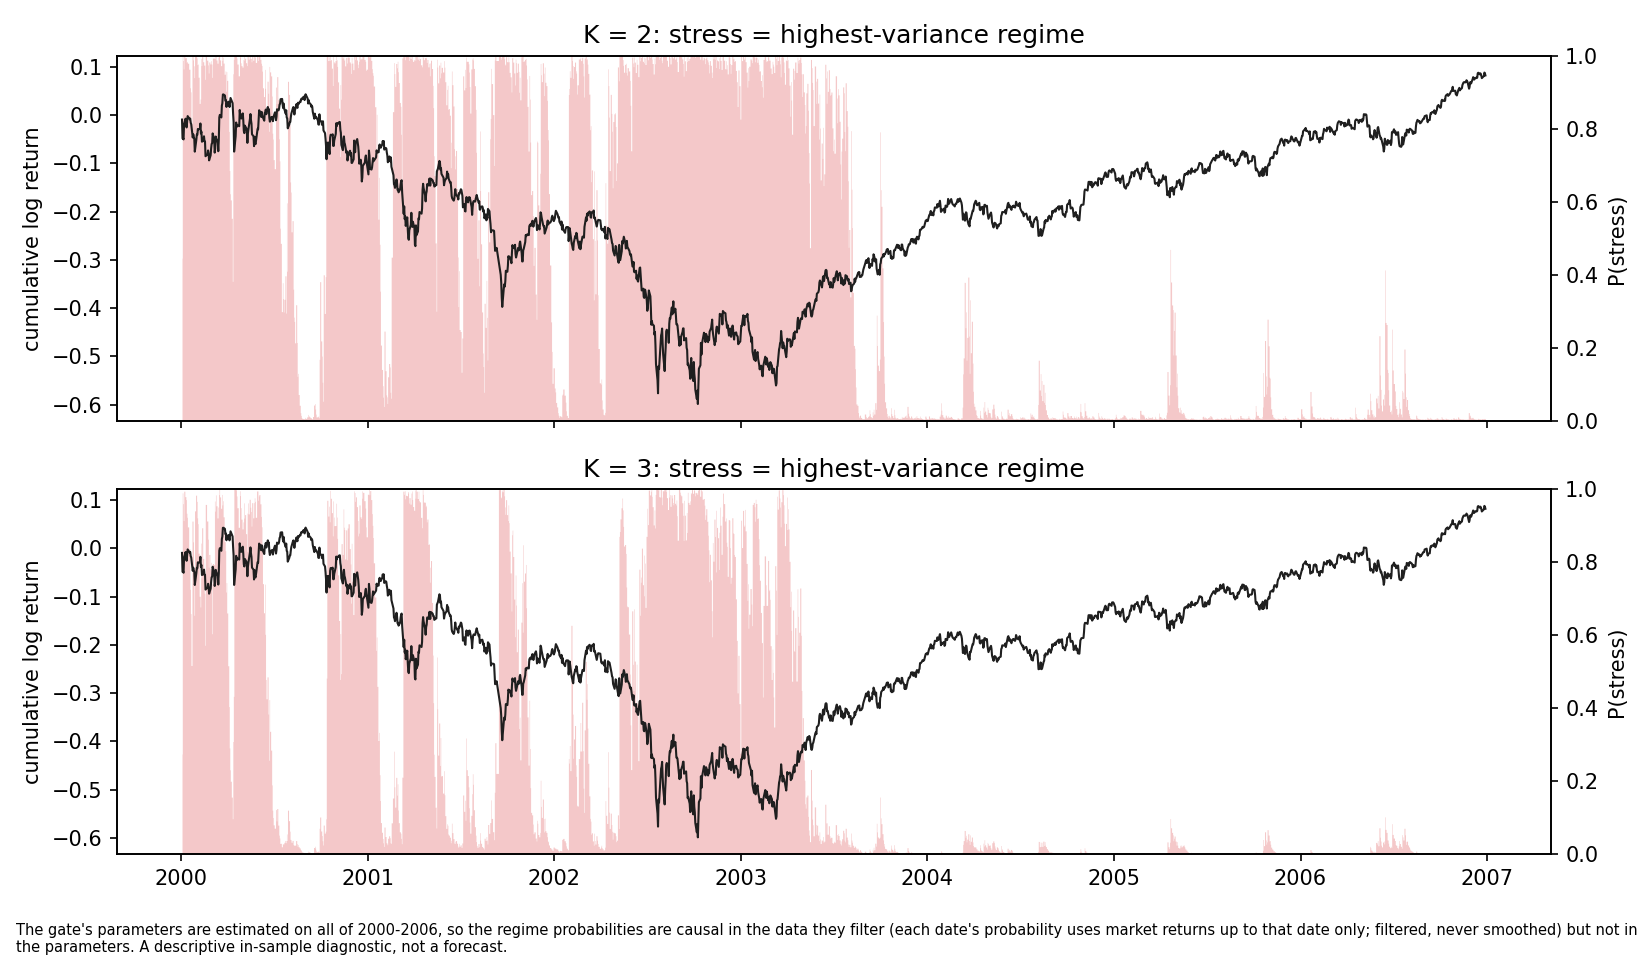
\includegraphics[width=0.92\textwidth]{fig/market_regimes_2000_2006.png}
\end{center}

\begin{itemize}
\item \textbf{$K=2$: one long stress block}, January 2000 to August 2003, calm afterwards. Daily volatility 0.69\% calm
  against 1.53\% stress; expected durations 229 and 177 days; all 24 starting points converged to the same optimum.
\item \textbf{$K=3$}: volatilities 0.60\%, 0.98\% and 1.75\%, expected durations 110, 46 and 79 days, so the stress state
  breaks into episodes inside 2000--03.
\end{itemize}

\begin{warnbox}{What this means for the next study}
With $K=2$ the regime contrast is largely ``2000--03 against 2003--06''. Any slow change in how a signal worked over
those years lands inside the ``regime'' contrast. This is the slow-drift case of the synthetic size check, where both
t-statistics over-reject. The trailing-volatility split switches far more often and is less tied to the 2003 break,
which is why it is the key robustness check below.
\end{warnbox}

\subsection{The IC split by regime}

\paragraph{Method (brief 11 B).} 18 signals (the 16 above plus within-industry reversal and industry momentum) at
$h=1$--$10$. For each date the gate gives regime weights $w_k(t)$ summing to one. Two estimates per regime:
\begin{itemize}
\item a \textbf{weighted mean IC}, $\sum_t w_k(t)\,\mathrm{IC}_t / \sum_t w_k(t)$, with its effective number of dates;
\item a \textbf{pure-regime IC} $c_k$ from the regression without intercept
  \[\mathrm{IC}_t=\sum_k c_k\,w_k(t)+e_t,\]
  the IC on a day fully in regime $k$. The \textbf{contrast} is $c_{\text{stress}}-c_{\text{calm}}$, with sandwich
  standard errors under two HAC choices: Hansen--Hodrick at lag $h-1$ and Newey--West at lag $\max(h-1,20)$, the
  second because a persistent regime probability makes residuals correlated beyond the target overlap.
\end{itemize}
Robustness: filtered instead of window weights, a hard split (weight above 0.5), and the trailing-volatility state.

\paragraph{Pre-specified tests.} Fixed before the run from the literature, at $K=2$, $h=5$, Hansen--Hodrick, one-sided,
with a Holm correction across the five:
\begin{itemize}
\item \textbf{H1} reversal is stronger in stress, for one-week, one-month and within-industry reversal (Nagel 2012;
  Hameed \& Mian 2015);
\item \textbf{H2} momentum is weaker in stress, for stock and industry momentum (Cooper, Gutierrez \& Hameed 2004;
  Wang \& Xu 2015; Daniel \& Moskowitz 2016).
\end{itemize}
Everything else is an exploratory family with Benjamini--Hochberg q-values.

\paragraph{Results: the five primary tests ($K=2$, $h=5$, window weights).}\mbox{}\par\smallskip

\begin{center}{\small
\begin{tabular}{@{}lrrrrr@{}}
\toprule
Signal & IC calm & IC stress & Contrast & $t$ (HH) & Holm $p$\\
\midrule
\texttt{ret\_5d} & $-1.70$ & $-3.46$ & $-1.76$ & $-1.31$ & 0.38\\
\texttt{ret\_20d} & $+0.20$ & $-3.83$ & $-4.03$ & $-2.17$ & 0.076\\
\texttt{ret\_20d\_ind\_rel} & $-0.74$ & $-2.19$ & $-1.45$ & $-1.11$ & 0.40\\
\texttt{mom\_12\_1} & $+2.83$ & $-0.07$ & $-2.90$ & $-1.10$ & 0.40\\
\texttt{ind\_mom\_12\_1} & $+0.58$ & $+0.74$ & $+0.17$ & $0.07$ & 0.53\\
\bottomrule
\end{tabular}}\end{center}
ICs and contrasts in percent.

\paragraph{Robustness of the contrasts (t-statistics, $h=5$).}\mbox{}\par\smallskip

\begin{center}{\small
\begin{tabular}{@{}lrrrrr@{}}
\toprule
Signal & $K{=}2$ HH & $K{=}2$ NW & $K{=}2$ hard & $K{=}3$ HH & Volatility split\\
\midrule
\texttt{ret\_5d} & $-1.31$ & $-1.43$ & $-1.28$ & $-1.43$ & $-0.68$\\
\texttt{ret\_20d} & $-2.17$ & $-2.42$ & $-1.89$ & $-3.05$ & $-2.16$\\
\texttt{ret\_20d\_ind\_rel} & $-1.11$ & $-1.24$ & $-0.83$ & $-1.78$ & $-1.27$\\
\texttt{mom\_12\_1} & $-1.10$ & $-1.13$ & $-1.17$ & $-1.23$ & $-0.96$\\
\texttt{ind\_mom\_12\_1} & $0.07$ & $0.08$ & $0.12$ & $-0.41$ & $0.43$\\
\bottomrule
\end{tabular}}\end{center}

\begin{center}
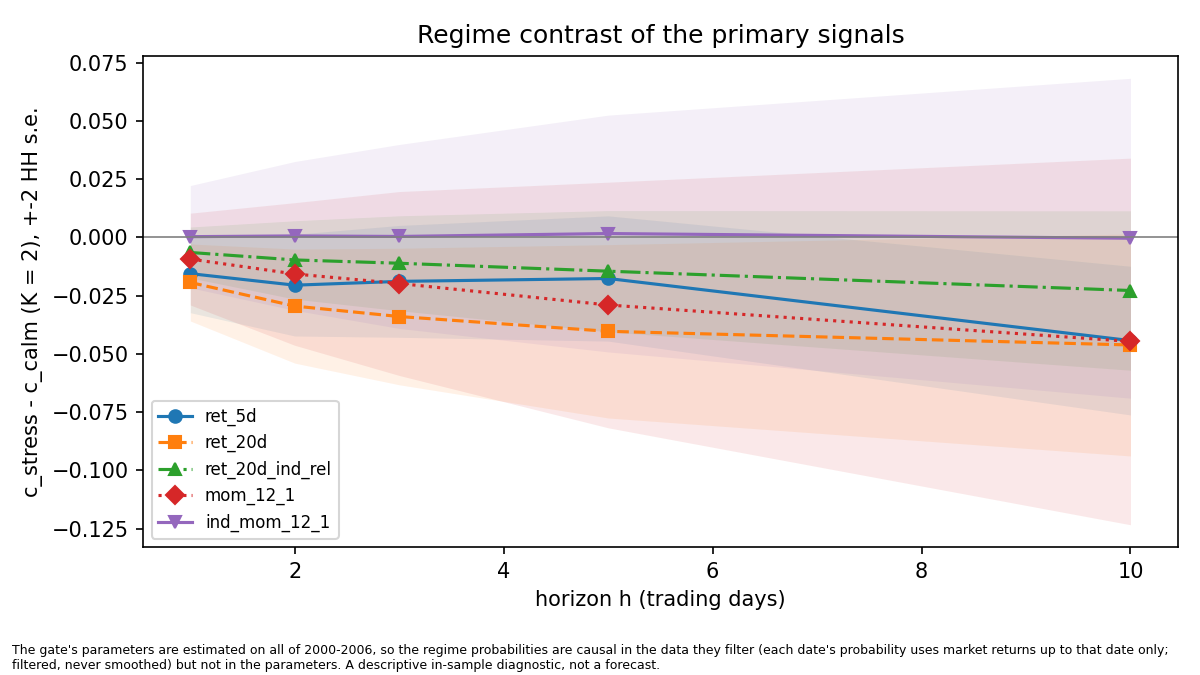
\includegraphics[width=0.78\textwidth]{fig/ic_regime_contrast_2000_2006.png}
\end{center}

\paragraph{Findings.}
\begin{itemize}
\item \textbf{The pattern matches the literature but is underpowered.} Four of five contrasts have the expected sign:
  one-week reversal is about twice as strong in stress, one-month reversal exists \emph{only} in stress, momentum
  works in calm and disappears in stress; industry momentum does not move. None survives Holm (smallest adjusted
  $p$ 0.076).
\item \textbf{One-month reversal is not just the 2003 break}: it keeps its contrast under the trailing-volatility
  split ($t=-2.16$) and is stronger at $K=3$ ($t=-3.05$). One-week reversal's contrast weakens under the volatility
  split ($-0.68$), so part of it may be drift.
\item \textbf{Exploratory family}: 11 of 175 contrasts reach $q<0.10$, none $q<0.05$. They are mainly abnormal volume
  (a stronger signal in stress at $h=3$--10, both $K$) and one-month reversal at $K=3$. These are hypotheses for
  2007--2024, not findings.
\end{itemize}

\begin{decbox}{Reading, by the rule written before the run: neutral}
Contrasts of the expected sign but not significant after Holm: consistent with the literature and with the
thesis's premise, but underpowered, because 2000--2006 contains essentially one long stress episode. The design is
unchanged. Regime dependence is tested properly where it matters: across the six stress episodes of 2010--2024 and
the 2008 crisis in the pilot years.
\end{decbox}

\subsection{Do sectors have their own regimes? (input to Q28)}

\paragraph{Method (brief 11 C).} For each GICS sector, the value-weighted daily return of its S\&P 500 members, as a
log return, both raw and \textbf{sector-relative} (sector minus index). A two-state Hamilton gate per sector and
series on 2000--2006, filtered probabilities. Measures: the share of days a sector is stressed while the market is
calm, the conditional probability of sector stress given market calm, the correlation of each sector's stress
probability with the market's, durations and episodes. Pre-written expectation: raw sector regimes largely copy the
market's; sector-relative ones should not.

\begin{center}
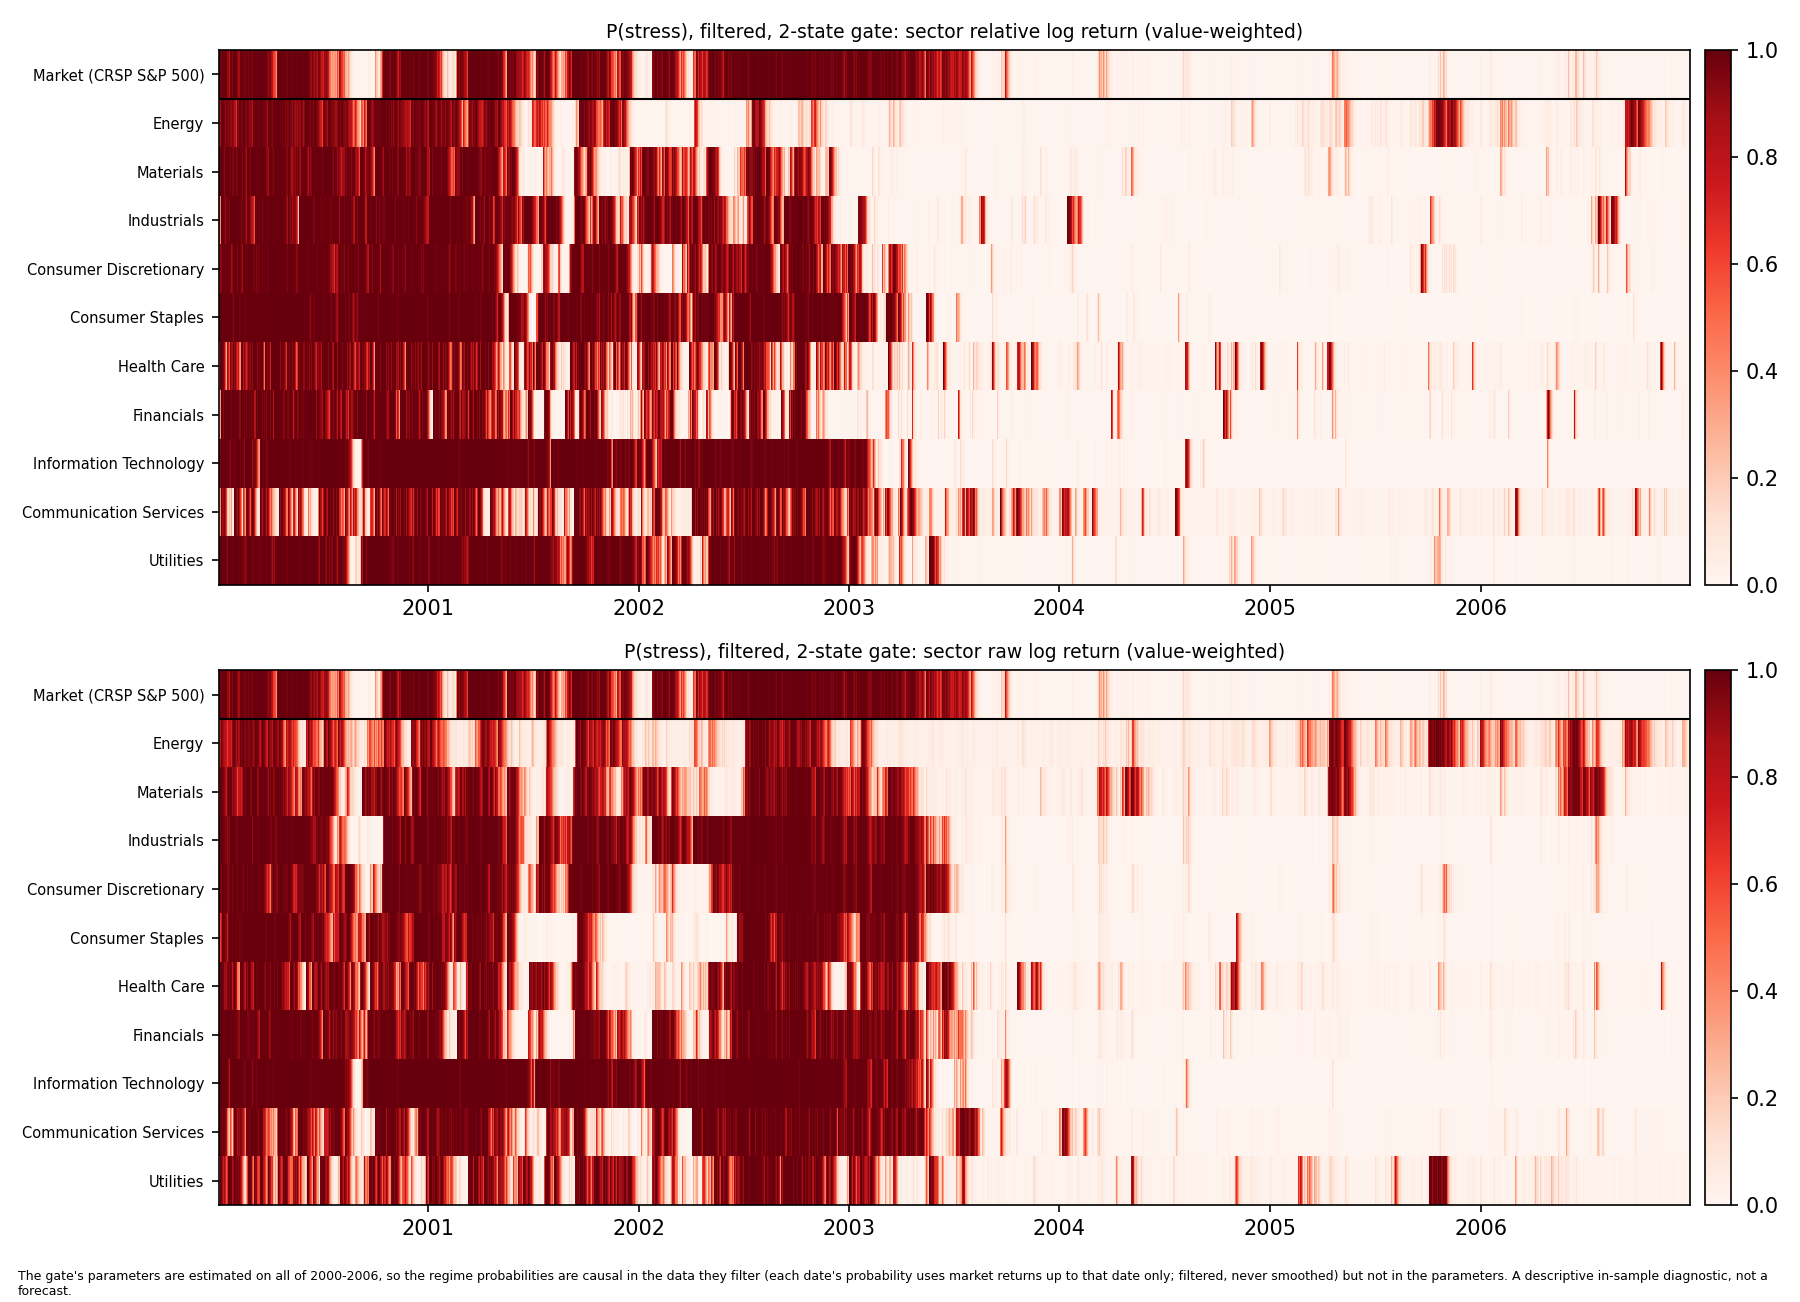
\includegraphics[width=\textwidth]{fig/sector_regimes_2000_2006.png}
\end{center}

\begin{center}\resizebox{\textwidth}{!}{%
\begin{tabular}{@{}lrrrrr@{}}
\toprule
Sector (relative, value-weighted) & Stressed & Stressed, market calm & P(stress $\mid$ calm) & Corr.\ with market & Episodes\\
\midrule
Energy & 28\% & 7.7\% & 13.7\% & 0.42 & 12\\
Materials & 30\% & 6.1\% & 10.8\% & 0.56 & 17\\
Industrials & 40\% & 9.3\% & 16.4\% & 0.61 & 16\\
Consumer Discretionary & 37\% & 5.8\% & 10.3\% & 0.70 & 13\\
Consumer Staples & 44\% & 7.0\% & 12.4\% & 0.80 & 11\\
Health Care & 37\% & 8.4\% & 14.8\% & 0.60 & 33\\
Financials & 30\% & 5.9\% & 10.5\% & 0.55 & 22\\
Information Technology & 44\% & 7.3\% & 13.0\% & 0.77 & 7\\
Communication Services & 35\% & 6.5\% & 11.5\% & 0.66 & 34\\
Utilities & 41\% & 6.4\% & 11.3\% & 0.77 & 9\\
\bottomrule
\end{tabular}}\end{center}

Real Estate has no names before 2016 (it was part of Financials) and was not fitted. Communication Services is the
thinnest sector (median 12 names, minimum 8).

\paragraph{Findings: between the two pre-written outcomes.}
\begin{itemize}
\item \textbf{Relative regimes follow the market less than raw ones, but still substantially}: median correlation with
  the market's stress probability 0.64 for relative series against 0.76 for raw. In the heat strips, relative stress
  mostly marks 2000--03, when sector returns diverged widely.
\item \textbf{Sector-own stress exists but is concentrated}: a sector is stressed while the market is calm on 6--9\% of
  days (conditional probability 10--16\%). The clearest sector-own episode is Energy in 2005--06, with sporadic
  Health Care and Communication Services spikes.
\item \textbf{Caveat}: the index contains the sector, so ``sector minus index'' partly cancels the largest sectors
  (technology was a fifth to a third of the index in 2000). A sector-minus-rest-of-market series would remove this.
\end{itemize}

\begin{openbox}{What this does and does not settle for Q28}
It informs the sub-questions on what the industry chain is fitted on (relative series are less market-driven but
need the cancellation fixed), granularity (thin sectors), and the descriptive check itself. It does \emph{not} choose
the form of the industry-level gate, which stays open; the 2000--2006 window has one market stress block, so the
co-movement of sector and market regimes may look different over 2007--2024.
\end{openbox}

\section{Compute budget}
\label{sec:compute}

\subsection{Machine and measurements}

Planning is done for Tom's laptop (Apple M4 Pro: 10 performance and 4 efficiency cores, 48\,GB) until a
school compute node is confirmed. \dec{2026-10-05}

\begin{whybox}[Why budget compute first]
The advisor's instruction was that compute is the binding constraint and that architecture choices are
settled only once the budget is calculated, not guessed. Planning on the laptop is the conservative case: if
the design fits there, a school node only adds slack. Everything was measured, not assumed: a synthetic
benchmark of every configuration, then one timed run on the real pipeline to measure the overhead.
\end{whybox}

\begin{itemize}
\item \textbf{Cost of one run.} With a fixed step budget, a run costs about
  \[\text{steps}\times\text{batch}\times(6P-2\,d\,w_1)\ \text{FLOPs},\]
  where $P$ is the number of parameters, $d$ the input dimension and $w_1$ the first width (the first
  layer needs no gradient with respect to its inputs). It does not depend on how many training rows
  there are.
\item \textbf{One thread per run}: a single core reaches 30--230 GFLOP/s; for $K=3$, widths 64--32, batch
  4,096: 238 steps/s. More threads in one run give nothing.
\item \textbf{Parallel runs}: 10 runs on the performance cores give 6.9$\times$ (7.6$\times$ with the
  efficiency cores). Plan: 10 parallel processes.
\item \textbf{GPU (MPS)}: a fixed 1.6--3\,ms per step; useful only for the largest models.
\item \textbf{Real pipeline} (timed 6 October on the 2009 pilot fold, 1.13M training rows): 5.57\,ms per
  step against the benchmark's 4.19\,ms, an overhead factor of 1.33. Gate fit 29\,s (Hamilton, $K=3$,
  24 starts), base fit 0.2\,s, peak memory 3.9\,GB.
\end{itemize}

\subsection{What the design costs}

One run trains one model for one fold from one seed. The design multiplies:

{\small
\begin{tabularx}{\textwidth}{@{}X X r@{}}
\toprule
Block & Count & Runs\\
\midrule
Gate $\times$ depth grid & 6 arms (5 gates + no-regime control) $\times$ 10 seeds $\times$ 15 folds & 900 per depth\\
Primary cell, extra seeds & 20 seeds $\times$ 15 folds & 300\\
Construction arms & 5 arms $\times$ 10 seeds $\times$ 15 folds & 750\\
Base depth sweep & 10 seeds $\times$ 15 folds & 150 per depth\\
Pilot & about 50 settings $\times$ 3 folds $\times$ 3 seeds & 450\\
No-decay arm for every gate & $6\times10\times15$ & 900\\
Leave-one-episode-out & primary cell & about 30\\
\bottomrule
\end{tabularx}}

Depths 1--3: 5,580 clean runs; budgeted twice for reruns. Laptop time with 10 parallel runs:

{\small
\begin{tabular}{@{}lllrrr@{}}
\toprule
Depths & $K$ & First width & 3k steps & 10k steps & 30k steps\\
\midrule
1--3 & 3 & 64 & 7\,h & 23\,h & 71\,h\\
1--3 & 3 & 128 & 14\,h & 46\,h & 137\,h\\
1--3 & 4 & 64 & 9\,h & 30\,h & 91\,h\\
1--3 & 4 & 256 & 38\,h & 126\,h & 377\,h\\
1--5 & 4 & 256 & 58\,h & 194\,h & 581\,h\\
\bottomrule
\end{tabular}}

\dec{2026-10-05} \textbf{Envelope: depths 1--3, first width at most 128, $K$ at most 4.} Within it the whole
study, run twice, takes about 1--2 days at 10,000 steps per run and 3--6 days at 30,000, plus up to half
a day of gate fits. Compute is therefore not the binding limit inside the envelope; the statistical
limit is (Q17, Q18). Still to confirm: steps per run (from the pilot), the fit times of the jump,
Wasserstein and TVTP gates, the industry-level gate fits (Q28), and thermal slowdown over multi-day
runs.

\begin{whybox}[Why this envelope]
Inside it, the whole design (every gate, depth, seed and fold, run twice) takes days, not months, so
compute stops being the constraint and the remaining choices can be made on statistical grounds (Q17,
Q18). Outside it, the only configurations ruled out are deep (4--5 layers) and wide (256) networks with
long training, which would take about a month and which the literature gives no reason to expect to help:
Gu, Kelly \& Xiu find shallow networks suffice. Counting every arm twice allows for bugs and reruns, which
in practice double the clean count.
\end{whybox}


\section{Implementation status}
\label{sec:status}

The code lives in \texttt{nec\_baseline} (package \texttt{nec\_moe}). Each block of decisions is turned into
a written code brief and implemented by Claude Code, with tests pinning every claim.

{\small
\begin{tabularx}{\textwidth}{@{}l X l@{}}
\toprule
Brief & Content & Status\\
\midrule
02 & Residual design: frozen base, zero-initialised experts, loss registry seam & done\\
03 & Gate interface (fit on the training block, apply causally) and the Hamilton gate & done\\
04 & Objective, multi-start fits, smoke runs & done\\
05 & Full code audit; critical findings fixed and pinned by tests & done\\
06 & CRSP data layer, S\&P 500 universe, delisting rule, provenance on every run & done\\
07 & Fixes, run store, exact resume, autoregressive Hamilton gate & done\\
08 & Market-neutral target, the 57-input feature set, point-in-time Compustat, GICS, window-average gate weight & done\\
09 & Sample 2000--2024, calendar-year folds, decay weights, native and weighted Baum--Welch, pilot runner,
parallel campaign runner, real-pipeline timing & done (commits f76f6eb--0e515eb)\\
10 & Gate filter through the purge gap (Q22), CRSP index as the gate series (Q23), IC decay script & done; IC decay run\\
11 & Regime-split IC curve and sector regimes on 2000--2006 (descriptive) & done; run 2026-10-09\\
12 & Evaluation additions: legs, decile monotonicity, years and episodes, execution lag & written, to run\\
\bottomrule
\end{tabularx}}

\subsection{What exists and what does not}

\begin{itemize}
\item \textbf{Built}: the 2000--2024 extracts and the point-in-time panel; feature coverage reports; the
  Hamilton and autoregressive Hamilton gates with the window-average weight and regime-clock memory;
  base and experts with decay weights; the per-row mixture likelihood; walk-forward evaluation with
  purge, Hansen--Hodrick statistics, the three NLLs and the long-short book; the pilot and campaign
  runners; the run store with exact resume.
\item \textbf{Not yet built}: the jump, Wasserstein and TVTP gates; the industry-level gate (waits on Q28);
  the diagnostics of Section~\ref{sec:evaluation} (decomposition, permutation test); the baselines beyond
  the existing priors (waits on Q12); the pre-registration document.
\item \textbf{Not yet run}: the pilot (run by Tom after review) and therefore every scored result.
\end{itemize}

\subsection{Documents}

\begin{itemize}
\item \texttt{Advisor\_Questions.md}: every question, open and resolved, with full reasoning.
\item \texttt{Progress\_Tracker.md}: current state, decision register, compute budget, log.
\item \texttt{MoE\_HMM\_Gate\_Formulation.pdf}: the mathematics (gate, EM, per-row likelihood, gate weight).
\item \texttt{Model\_Derivation\_BaseCase.md}: the base-case derivation.
\item \texttt{Training\_Window\_and\_Weighting\_Theory.md}: theory of the training window and weights.
\item \texttt{Improvements\_and\_Extensions.md}: future work: E1 one-day forecasting; E2 the MoE as a stacking
  meta-model over machine-learning alphas; E3 residual short-term reversal as an input; E4 recurrent or transformer
  experts on raw price sequences.
\end{itemize}
The formulation PDF and the derivation still describe one shared gate weight per date; they will get a
section on the industry-level gate once Q28 is settled.

\section{Open questions}
\label{sec:open}

Grouped by topic. Each entry says what has to be decided and why it matters; the full discussion is in
\texttt{Advisor\_Questions.md}.

\subsection{Gate design}

\begin{openbox}{Q28. How is the industry-level gate implemented?}
Q1 fixed the direction (market regime combined with an industry regime, both frozen). Open: the form
(factorial, coupled chains, sector-only, pooled chains), what the industry chain is fitted on
(sector-relative or raw sector returns), granularity (11 sectors or finer), states per level, how each
gate type gets an industry version, and identification against the industry inputs. Section~\ref{sec:industrygate}. The descriptive check on 2000--2006 (Section~\ref{sec:diagnostics}) found sector-own stress on 6--9\% of days,
concentrated in a few sectors, with relative regimes still correlated 0.64 with the market's.
\end{openbox}

\begin{openbox}{Q29. A gate defined by factor returns?}
A gate variant whose observation is the vector of daily factor returns (market, size, value, momentum),
so regimes describe how the cross-section behaves. Open: a sixth gate type or an input to an existing
one; which factors; built from the panel or French's factors; full or simplified covariance; how it
relates to Q28.
\end{openbox}

\begin{openbox}{Q13. Should a recurrent gate be added?}
A GRU router has memory without a regime process. Without such an arm, a win for regime gates over
memoryless references cannot tell ``memory helps'' from ``regime structure helps''.
\end{openbox}

\subsection{Model size and structure}

\begin{openbox}{Q18. How many regimes, $K$?}
$K$ is an input to every gate and is held fixed across gates (no sweep). The data cap it: what counts
is the number of regime episodes, not days, and an over-specified mixture is estimated far more slowly.
With the industry-level gate it may become two numbers. Must be argued, not tuned.
\end{openbox}

\begin{openbox}{Q17. What can learning theory say about network size?}
Classical VC bounds are vacuous at this scale (bounds of order 0.5 against an attainable $R^2$ of about
0.004). Whether another strand (e.g.\ norm-based or PAC-Bayes bounds) gives a usable argument, or the
size is set by the envelope and the pilot.
\end{openbox}

\begin{openbox}{Q8. Widths inside the envelope}
Depths 1--3, first width at most 128, pyramid rule. Which first width, and how the capacity-matched
baseline is sized.
\end{openbox}

\begin{openbox}{Q6 (design half) and Q14. The residual construction}
Whether ``we chose the architecture that isolates the variable under study'' is enough justification
for the residual design on a returns target; whether the experts are held to small corrections by a
shrinkage penalty $\alpha$ (untested in the literature) or only by zero initialisation; the role of the
five construction arms.
\end{openbox}

\subsection{Training and evaluation}

\begin{openbox}{Q20. The error function}
Mixture likelihood (current), squared or Huber error on the point forecast, or a rank/IC objective.
Under a frozen gate the likelihood lets the realised target re-weight experts after the gate has
assigned them; squared error does not. Also decides what the noise scales mean.
\end{openbox}

\begin{openbox}{Q12. Baselines}
Which of: capacity-matched network, one-expert network, penalised linear model, gradient-boosted trees,
no-gate mixture, jointly trained priors.
\end{openbox}

\begin{openbox}{Q9. Primary metric family}
Forecast accuracy (rank IC, ICIR) or portfolio performance; they can disagree, so one must be primary,
fixed in advance. Also open: whether transaction costs enter headline results (Q9 (c)). The reporting additions
(legs, deciles, years and episodes, execution lag) are decided.
\end{openbox}

\begin{openbox}{Q15. Adaptive overfitting}
The formal multiple-testing correction across the gate-by-depth grid and the pre-registration document.
\end{openbox}

\begin{openbox}{Q10. Is the frozen base really isolated?}
Which diagnostics are reported as evidence that the correction term is regime-conditional and not
relearned general signal, and whether a structural option is needed.
\end{openbox}

\begin{openbox}{Q16 (c). Leave-one-episode-out}
Whether training without a crisis and testing on it is a headline result or a robustness check.
\end{openbox}

\subsection{Positioning}

\begin{openbox}{Q5. Positioning against Ye \& Borde (2026)}
Their RG-ResMoE has no regime model (its ``regime'' is two rolling volatilities fed to a learned gate)
and predicts volatility, not returns. Adopting their architecture leaves the contribution in the gate.
Open: whether adopting a very recent paper's architecture wholesale is acceptable, clearly attributed.
\end{openbox}

\subsection{Smaller open items}

\begin{itemize}
\item The long-short book's default scheme (non-overlapping or staggered).
\item The hidden-layer initialisation of the experts (audit X-1).
\item The experts' regime-clock decay as a mixture over regimes (default) or per expert.
\item Clipping outliers in the training target (held for later, with Q20).
\item The post-delisting fill (``cash'' default, not a decision).
\item Restated Compustat values: whether the ``prior to amendment'' keysets fix them.
\end{itemize}

\subsection{A suggested order}

\begin{enumerate}
\item \textbf{Q18 with Q28}: $K$ and the industry-gate form decide the number of experts and what gets
  built next.
\item \textbf{Q20}: the loss changes what every run optimises.
\item \textbf{Q12 and Q9}: what results mean, fixed before any are seen.
\item \textbf{Q8, Q6/Q14, Q17}: sizes and construction inside the envelope.
\item \textbf{Q15}: pre-registration, after which the pilot is run.
\item Q29, Q13, Q16 (c), Q5, Q10 alongside, as they do not block the pilot.
\end{enumerate}

\section{Decision register}
\label{sec:register}

Every big decision since the advisor meeting of 18 September 2026, oldest first, copied from
\texttt{Progress\_Tracker.md} (section 1b). ``Instead of'' records what the decision replaced or rejected.

{\footnotesize
\begin{longtable}{@{}p{1.55cm}>{\raggedright\arraybackslash}p{6.6cm}>{\raggedright\arraybackslash}p{4.2cm}>{\raggedright\arraybackslash}p{2.6cm}@{}}
\toprule
Date & Decision & Instead of / why & Where\\
\midrule
\endhead
2026-09-18 & Data is CRSP (US equities); Wind only as a possible China extension & free data & Q3; advisor meeting\\
2026-09-18 & Report the full mechanism-by-depth grid, nothing tuned away; depths set by the compute budget & fixing or tuning depth & Q11; advisor meeting\\
2026-09-18 & No width sweep: widths follow the pyramid rule from a fixed first layer & sweeping widths & advisor meeting\\
2026-09-18 & No sweep over K: K fixed by argument and held across all gates & sweeping K & advisor meeting; K itself is Q18 (open)\\
2026-09-18 & Order of work: data, then compute budget, then parameters; start with the base and a generic loss & designing the loss first & advisor meeting\\
2026-09-21 & Gate fitted separately and frozen, for every gate & joint training & Q19\\
2026-09-21 & Base pre-trained and frozen; experts are corrections to it (residual design) & joint training & Q7; brief 02\\
2026-09-26 & CRSP replaces free price and universe data everywhere & yfinance/Stooq/Wikipedia & brief 06\\
2026-09-26 & S\&P 500 universe from CRSP membership INDNO 1000500, bounds inclusive & 1000502 (no constituents) & brief 06 A.3 erratum\\
2026-09-26 & Delisting rule (a): CIZ DlyRet already contains the delisting return & compounding DelRet in & brief 06\\
2026-09-26 & Overlapping-target t-statistics: Hansen-Hodrick & Newey-West (worse size in simulation) & audit E-2\\
2026-09-26 & Report the volatility-only NLL gain next to the correction gain & one combined number & audit E-1 follow-up\\
2026-10-01 & Target: market-neutral return (forward return minus the date's equal-weighted cross-sectional mean) & raw, CAPM residual, standardised, vol-scaled & Q25\\
2026-10-05 & All reporting on the market-neutral basis, no raw-return reporting & reporting raw returns too & Q25 clarification\\
2026-10-05 & Daily gate, daily cross-section, 5-day target (option B) & h = 1, monthly & Q21\\
2026-10-05 & Features: two representatives per JKP theme plus a 6-theme short-horizon market block and an industry block; 40 characteristics, 57 inputs & the 14 legacy price features & Q26\\
2026-10-05 & Ranks mapped to [-1, 1] & [-0.5, 0.5] & Q26 part 2\\
2026-10-05 & Missing values: minimum-count windows, fundamentals carried forward for at most 12 months, then 0 plus a flag per family; rows no longer dropped & dropping rows; interpolation (look-ahead) & Q26 part 3\\
2026-10-05 & Industry: sector dummies, within-sector ranks of 4 fundamentals, industry momentum and within-industry reversal & none, or a subset & Q26 part 4\\
2026-10-05 & Sector source: GICS from Compustat & ICB (CRSP stops filling it in Oct 2023) & Q26 part 4\\
2026-10-05 & Point-in-time fundamentals: usable the trading day after the later of report and filing date; surprises dated by the report date & quarter end plus a lag & Q26 part 5; brief 08 C\\
2026-10-05 & IVAOQ, IVSTQ, MIBQ, PSTKQ count as 0 when blank in total accruals and net operating assets & strict "missing" (left those features on about 5\% of rows) & commit 5524da1 (after the first coverage report)\\
2026-10-05 & Experts trained on the per-row likelihood, read as the composite (independence) likelihood of the per-date model & per-date likelihood & Q24; PDF Appendix D\\
2026-10-05 & Gate weight for the 5-day target: average of the 1- to 5-step-ahead regime probabilities & filtered or one-step predicted & Q27; PDF Section 8.9\\
2026-10-05 & Backprop-HMM baseline keeps its own h-step predict & moving it to window weights & Q27 correction\\
2026-10-05 & Sample 2000--2024 & 2015--2024 (too few stress episodes) & Q16 (a)\\
2026-10-05 & Expanding training window & rolling & Q16 (b)\\
2026-10-05 & Experts: regime-clock decay (age = later same-regime experience; one half-life in regime-days) & equal weights; calendar decay (erases crises) & Q16 (d)(e); \url{Training_Window_and_Weighting_Theory.md}\\
2026-10-05 & Base: calendar exponential decay, long half-life & equal weights & Q16 (d)\\
2026-10-05 & Gate: regime-clock forgetting via a two-pass weighted Baum-Welch; memory chosen by one-step predictive log-likelihood on validation & full history; calendar forgetting (can lose the stress state) & Q16 (d)(e); theory notes section 7\\
2026-10-05 & Every half-life chosen once from a preset grid (equal weights always included) in the pilot on early validation blocks, then frozen and pre-registered & tuning per fold or on test data & Q16; Q15\\
2026-10-05 & Compute planning on the laptop (Apple M4 Pro, 48 GB) until the school node is confirmed & -- & this log\\
2026-10-05 & Test period 2010--2024, refitted annually (15 folds) & testing from 2008 (pilot would see no crisis) & Q16\\
2026-10-05 & Pilot on validation years 2007--2009 chooses every setting once (half-lives, gate memory, learning rate, weight decay, step budget), with a regime-balanced validation loss; then frozen and pre-registered & tuning in every fold; a calm-only validation & Q16; Q15\\
2026-10-05 & Main study trains on the full block: no held-out tail, no per-fold early stopping (resolves B-2); fallback to regime-balanced early stopping if the pilot's best step budget drifts & the last-20\% validation tail & Q16; audit B-2\\
2026-10-05 & Train on every day under a fixed step budget & every 5th day (saves nothing under a step budget) & Q16\\
2026-10-05 & Fresh initialisation every fold; warm starts only as a fallback (shrink and perturb) & warm starts (worse generalisation; break zero-init residual design) & Q16; Ash \& Adams 2020\\
2026-10-05 & Seeds paired across arms; 10 per grid cell, 30 for the primary cell, final count from the pilot's measured seed variance & independent seeds per arm & Q16; Q11\\
2026-10-05 & Engineering: one process per performance core, large batches fixed in the pilot, features built once, base cached & default single-process training & Q16\\
2026-10-05 & Compute envelope for the design: depth scan 1--3 (pyramid widths from a fixed first width), first width at most 128, K at most 4; runs on the laptop, 10 parallel processes & depths 1--5 and first width 256 (1--1.5 months of laptop time; Gu, Kelly \& Xiu find depths 4--5 add nothing) & section 1c; Q8, Q11\\
2026-10-05 & Brief 09 written: implements the sample extension, calendar-year folds, the pilot, decay weights, the weighted Baum-Welch gate, the parallel runner & -- & \url{Code_Change_Brief_09_Training_Scheme.md}\\
2026-10-08 & The gate's filter runs over every trading day, including the purge gap; parameters still fitted on training only & skipping the gap (one step of A bridged 6 days) & Q22\\
2026-10-08 & Gate input: CRSP value-weighted S\&P 500 universe index (1000500), daily log total return; French Mkt-RF kept as a robustness check & French Mkt-RF (external file, whole market) & Q23\\
2026-10-08 & Gate is partly stock-specific at the industry level: market regime combined with an industry-level regime, both frozen; how it is implemented is open (Q28) & one market-wide weight vector per date & Q1, Q28\\
2026-10-08 & Framing: comparison-led; no constructive element (the differentiable jump-model gate is not pursued) & adding a design-led contribution & Q2, Q4\\
2026-10-08 & Horizon stays h = 5; add an IC decay curve on 2000--2006 and a horizon profile (h = 1, 3, 5, 10) for the final model as robustness & switching to h = 3 or h = 1 & Q21 follow-up\\
2026-10-09 & IC decay curve (2000--2006) confirms h = 5: one-week reversal and abnormal volume peak at 5, slow signals still build, nothing favours 3; horizon question closed; Q26 inputs unchanged despite weak pooled ICs & switching horizon; pruning weak signals on outcomes & Q21 follow-up result\\
2026-10-09 & Reporting additions for every arm: long-leg vs short-leg returns and half-sample ICs; decile monotonicity (Patton-Timmermann test); IC by year and by 8 pre-named episodes; execution\_lag knob, headline tables at L = 0 and 1 & headline IC and long-short only & Q9 update; brief 12\\
2026-10-09 & Residual short-term reversal (resid\_mom20) kept as an extension, not added to the inputs (pilot already run) & changing Q26 after the pilot & Improvements E3\\
\bottomrule
\end{longtable}}

\appendix
\section{Glossary}

\begin{description}[style=nextline,leftmargin=1.2cm,itemsep=3pt]
\item[MLP (multilayer perceptron)] A feed-forward neural network: layers of weighted sums followed by a
  nonlinearity (here ReLU). Depth is the number of hidden layers, width the number of units per layer.
\item[Mixture of experts (MoE)] Several sub-models (experts) whose outputs are combined with weights from
  a gate. Here the experts are corrections to a base network and the gate is a regime model.
\item[Residual design] The experts learn corrections to a frozen base, starting from zero, instead of
  full forecasts.
\item[Gate, regime] A model that assigns probabilities to a small number of market states (regimes),
  such as calm and stressed.
\item[Hidden Markov model (HMM), Hamilton model] A model in which an unobserved state follows a Markov
  chain and the observed series is drawn from a state-specific distribution. Hamilton's (1989) Markov
  switching model is the econometric version.
\item[Filtered probability] The probability of today's regime given data up to today, $\xi_{t\mid t}$. The
  \emph{smoothed} probability also uses future data and is never used.
\item[Transition matrix $A$] The probabilities of moving from each regime to each other regime in one day.
\item[EM, Baum--Welch] The expectation--maximisation algorithm; Baum--Welch is EM for HMMs (forward
  filter, backward smoother, closed-form updates).
\item[Window-average gate weight] The expected share of the 5-day target window spent in each regime.
\item[Regime-clock decay] Down-weighting old observations by how much \emph{newer experience of the same
  regime} has accumulated, instead of by calendar age.
\item[Half-life] The age at which a weight has fallen to one half.
\item[Kish effective sample size] $(\sum w)^2/\sum w^2$: how many equally weighted observations a set of
  weights is worth.
\item[Rank IC (information coefficient)] The Spearman rank correlation, across stocks on a date, between
  forecasts and realised returns. ICIR is its mean divided by its standard deviation.
\item[Hansen--Hodrick standard errors] Standard errors that correct for overlapping observations (here,
  5-day targets sampled daily share four days).
\item[Purge] Dropping the last $h$ training days before a test block, because their targets reach into
  the test period.
\item[Walk-forward, expanding window] Repeated train-then-test in time order; the training block grows
  each fold.
\item[NLL] Negative log-likelihood: how improbable the realised targets are under the model's
  predictive distribution (lower is better).
\item[Composite likelihood] A product of marginal (here one-stock) likelihoods used in place of the full
  joint likelihood; consistent, with sandwich standard errors.
\item[Point-in-time] Using only the values that were known on the date, as first published, with report
  delays respected.
\item[Market-neutral return] A stock's return minus the cross-sectional average return on the same date.
\item[JKP themes] The 13 clusters of published stock characteristics in Jensen, Kelly \& Pedersen (2023).
\item[GICS] Global Industry Classification Standard; 11 sectors.
\item[Factorial HMM] Several independent hidden chains running in parallel, whose states combine.
\item[TVTP] Time-varying transition probabilities: a Markov switching model whose switching probabilities
  depend on observed covariates.
\item[Statistical jump model] Clustering of feature vectors over time with a penalty on switching
  between clusters, which makes regimes persistent.
\item[Pilot] The pre-2010 runs that choose every setting once, before the test period is touched.
\item[Pre-registration] Writing down the design, settings and primary comparisons before seeing test
  results.
\item[Paired seeds] Running every arm on the same random seeds and comparing seed by seed, which removes
  much of the noise from comparisons.
\end{description}

\section{References cited}

{\small
\begin{itemize}[leftmargin=*,itemsep=1pt]
\item Ash, J.\ \& Adams, R.\ (2020). On warm-starting neural network training. \emph{NeurIPS}.
\item Chordia, T., Subrahmanyam, A.\ \& Tong, Q.\ (2014). Have capital market anomalies attenuated in the
  recent era of high liquidity and trading activity? \emph{Journal of Accounting and Economics} 58.
\item Daniel, K.\ \& Moskowitz, T.\ (2016). Momentum crashes. \emph{Journal of Financial Economics} 122(2).
\item Diebold, F., Lee, J.-H.\ \& Weinbach, G.\ (1994). Regime switching with time-varying transition
  probabilities. In Hargreaves (ed.), \emph{Nonstationary Time Series Analysis and Cointegration}.
\item Filardo, A.\ (1994). Business-cycle phases and their transitional dynamics. \emph{JBES} 12(3).
\item Fischer, T.\ \& Krauss, C.\ (2018). Deep learning with LSTM networks for financial market
  predictions. \emph{European Journal of Operational Research} 270(2).
\item Ghahramani, Z.\ \& Jordan, M.\ (1997). Factorial hidden Markov models. \emph{Machine Learning} 29.
\item Gu, S., Kelly, B.\ \& Xiu, D.\ (2020). Empirical asset pricing via machine learning. \emph{Review of
  Financial Studies} 33(5).
\item Hamilton, J.\ (1989). A new approach to the economic analysis of nonstationary time series and the
  business cycle. \emph{Econometrica} 57(2).
\item Heinrich, P.\ \& Kahn, J.\ (2018). Strong identifiability and optimal minimax rates for finite
  mixture estimation. \emph{Annals of Statistics} 46(6A).
\item Jensen, T., Kelly, B.\ \& Pedersen, L.\ (2023). Is there a replication crisis in finance?
  \emph{Journal of Finance} 78(5).
\item Krauss, C., Do, X.\ \& Huck, N.\ (2017). Deep neural networks, gradient-boosted trees, random forests:
  statistical arbitrage on the S\&P 500. \emph{European Journal of Operational Research} 259(2).
\item McLean, R.\ \& Pontiff, J.\ (2016). Does academic research destroy stock return predictability?
  \emph{Journal of Finance} 71(1).
\item Mulliner, A., Harvey, C., Xia, C., Fang, E.\ \& Van Hemert, O.\ (2025). Regimes. \emph{Journal of
  Portfolio Management} 52(4).
\item Nagel, S.\ (2012). Evaporating liquidity. \emph{Review of Financial Studies} 25(7).
\item Nystrup, P., Madsen, H.\ \& Lindstr\"om, E.\ (2017). Long memory of financial time series and hidden
  Markov models with time-varying parameters. \emph{Journal of Forecasting} 36(8).
\item Pesaran, M.\ \& Timmermann, A.\ (2007). Selection of estimation window in the presence of breaks.
  \emph{Journal of Econometrics} 137(1).
\item Roll, R.\ (1984). A simple implicit measure of the effective bid-ask spread. \emph{Journal of
  Finance} 39(4).
\item Varin, C., Reid, N.\ \& Firth, D.\ (2011). An overview of composite likelihood methods.
  \emph{Statistica Sinica} 21.
\item Ye \& Borde (2026). Regime-gated residual mixture of experts (RG-ResMoE). arXiv:2608.12251.
\end{itemize}}


\end{document}
